\chapter{Higgs to WW$^*$ at 1.4 TeV}
\label{Higgs Analysis}

\begin{figure}
  \centering
  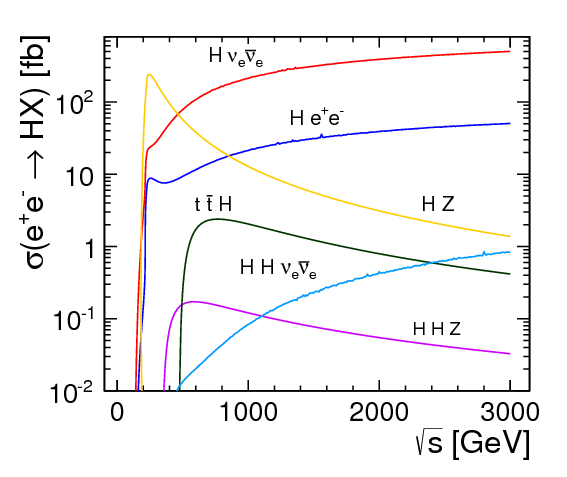
\includegraphics[width=0.7\textwidth,keepaspectratio]{Theory/fig/HiggsCrossSections}
  \caption[Cross Sections For Higgs Production Mechanisms]{Cross sections for dominant Higgs production mechanisms as a function of energy \cite{Abramowicz:2016zbo}. Higgs production via WW-fusion is shown in red.}
  \label{fig:higgsXSecs2}
\end{figure}

One of the key aims of the \ac{CLIC} physics programme will be to perform model independent measurements of the Higgs couplings. To enable this, the total width of the Higgs must first be measured. This is possible\cite{Durig:2014lfa} by taking the ratio of four different measurements


\hspace{120pt}  $X_1=\sigma_{ZH} \propto g_{HZZ}^2$,

\hspace{120pt}   $X_2=\sigma_{H\nu\bar{\nu}} \times BR(H\rightarrow WW^*) \propto \frac{g_{HWW}^4}{\Gamma_H}$,

\hspace{120pt}   $X_3=\sigma_{H\nu\bar{\nu}} \times BR(H\rightarrow b\bar{b}) \propto \frac{g_{HWW}^{2}g_{Hbb}^2}{\Gamma_H}$,

\hspace{120pt}   $X_4=\sigma_{ZH} \times BR(H\rightarrow b\bar{b}) \propto \frac{g_{HZZ}^{2}g_{Hbb}^2}{\Gamma_H}$.


Here we will look at the measurement of one of these, $X_2$. As can be seen from \reffig{fig:higgsXSecs2}, WW-fusion is the dominant Higgs production mechanism for energies above $\sim $500 GeV and so this measurement is best performed in the higher energy stages of operation. In particular we will focus on measuring $X_2$ at 1.4 TeV. For measuring the branching ratio of H$\rightarrow$WW$^*$ there are three potential final states that can be examined depending on the decay mode of the two W's. An individual W will decay hadronically (into a quark pair) 67.41\% of the time and leptonically (into a lepton + neutrino) 32.58\% of the time.  The combinations available from each W decay gives three final states referred to as the hadronic, semileptonic and leptonic decay modes corresponding to both W's decaying hadronically, one W decaying hadronically while the other decays leptonically and both W's decaying leptonically respectively. The relative abundance for each decay mode is roughly 4:4:1. Here we will only study the semileptonic mode (\reffig{fig:semileptonic}.) An equivalent analysis has already been performed for the hadronic decay mode yielding a statistical precision of 1.5\% on $X_2$ \cite{Abramowicz:2016zbo}. Due to its lower branching ratio, the leptonic decay mode has yet to be studied as it is not expected to yield a significant improvement on the statistical precision achievable for $X_2$. 

\begin{figure}
  \centering
  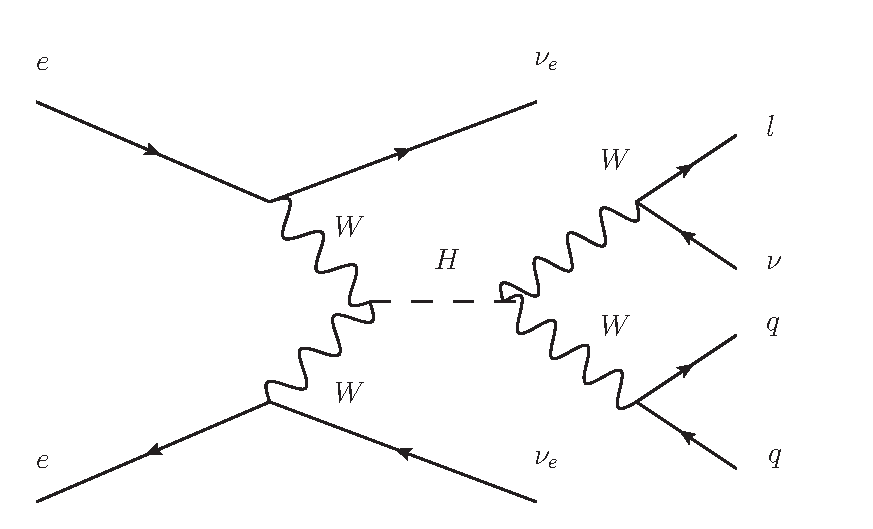
\includegraphics[width=0.7\textwidth,keepaspectratio]{HiggsAnalysis/figures/HiggsFeynman.eps}
  \caption[Semileptonic decay channel for  WW$^*$ decays of Higgs produced through WW-fusion]{Semileptonic decay channel for  WW$^*$ decays of Higgs produced through WW-fusion.}
  \label{fig:semileptonic}
\end{figure}

\section{Event Generation}

All events used in this analysis were produced centrally by \ac{CLIC} using WHIZARD 1.95 \cite{Kilian:2007gr} and are summarized in \reftab{fig:higgsbackgrounds}. In the case of $e\gamma$ events, a scale factor of 2 was applied to the cross section to account for interactions occurring with both the electron and positron. In the case of beamsstrahlung events (simulated using GUINEA-PIG \cite{Schulte:382453}), a further scaling of 0.75 was applied to account for the lower luminosity of these type of collisions. Sample 2022 is the $ee\rightarrow H\nu\nu$ inclusive sample and assumes a Higgs mass of $m_H = 126~GeV$. Events classified as signal were extracted from this main sample by performing a parton level event selection to identify events in which the Higgs decayed to W's and separating these according to their decay products. At this point events in which the lepton produced in the W decay is found to be a $\tau$ are excluded from the signal definition due to the fact they produce a different topology in the final state compared to electrons and muons as they are capable of producing jets in their decays. It is anticipated that a dedicated analysis would be used for identifying these events. In all cases the detector model used is CLIC\_ILD\_CDR, CLIC's variation of the ILD detector designed for ILC described in the \ac{CLIC} CDR\cite{CDR}. The main backgrounds of note are: ee$\rightarrow$qql$\nu$ (dominated by e$^+$e$^-\rightarrow$W$^+$W$^-$) as it has a very similar topology to the signal process and so is expected to be the most difficult to exclude; and ee$\rightarrow$ H(WW$^*\rightarrow$qqqq)$\nu\nu$ as contamination from these events after event selection must be taken into account before any combination of results from the semileptonic and hadronic channels can be made.


\begin{table}
  \centering
  \begin{tabular}{l r r r}
   \toprule
    Process     & Cross Section(fb)  &   Production ID\cite{bib-prodids}    & Events Used    \\
    \midrule
    Signal: ee$\rightarrow$ H(WW$^*\rightarrow$qql$\nu$)$\nu\nu$             &   17.3  &  2022  & 70000  \\ 
    \midrule
    ee$\rightarrow$ H(WW$^*\rightarrow$qqqq)$\nu\nu$                &   27.4  &  2022    & 100000 \\
    \midrule
    ee$\rightarrow$ H$^*\rightarrow$ Other & 199.4 & 2022 & 800000  \\
    \midrule
    ee$\rightarrow$qq               & 4009.5    &  2091  & 500000  \\ 
    \midrule
    ee$\rightarrow$qqqq               & 1328.1    &  2163  & 300000  \\ 
    \midrule
    e$\gamma$$\rightarrow$eqq ($\gamma$ from EPA)                 & 32308    &  2515 & 500000   \\ 
    \midrule
    e$\gamma$$\rightarrow$eqq ($\gamma$ from BS)               & 56043  &  2527  & 500000 \\ 
    \midrule
    ee$\rightarrow$qq$\nu\nu$               & 787.7    &  3243 & 500000   \\ 
    \midrule
    ee$\rightarrow$qqll               & 2725.8    &  3246  & 400000  \\ 
    \midrule
    ee$\rightarrow$qql$\nu$              & 4309.7    &  3249 & 1000000   \\ 
    \bottomrule
  \end{tabular}
  \caption[Samples used for the H$\rightarrow$WW$^*$ analysis]{Samples used for the H$\rightarrow$WW$^*$ analysis}
  \label{fig:higgsbackgrounds}
\end{table}


\section{Event Reconstruction}

Reconstruction of the signal events was performed using ILCSOFT v01-17-06 and was carried out in two main stages as described below. The first stage was to identify the isolated lepton associated with the leptonic W boson decay. The second stage involved removing this isolated lepton and resolving the remaining particles into two jets that were associated with the two quarks produced by the hadronically decaying W boson. Using the two jets, the W boson could then be reconstructed and combined with the isolated lepton to reconstruct the Higgs boson. The reconstructed Higgs candidate will not be complete due to the missing energy and momentum from the lepton neutrino produced from the W decay, where here the term missing refers to the difference between the nominal collision four momentum and the collective four momentum of the \ac{PFO}s recorded for the event. However, the observed properties will still be sufficient for providing discrimination between signal and background events.

\subsection{Lepton Identification}
Two different methods were used for identifying leptons. The primary method for particle identification is to assume that the highest energy electron or muon (as identified by PandoraPFA \cite{Thomson200925}) corresponds to the isolated lepton from the leptonically decaying W boson. This method was found to have an efficiency of 93\% (90\% for electrons, 96\% for muons) and purity of 96\% for identifiying the isolated lepton. The improved efficiency for muons relative to electrons is a result of the different signatures they leave in the detector. Electrons are identified by the presence of a track followed by a deposit in the \ac{ECAL}. If the track is not reconstructed or is attributed to the wrong calorimeter deposit by Pandora, the electron will be incorrectly identified as a photon (characterised by no track, only energy deposited in the \ac{ECAL}.) Muons on the other hand are highly penetrating and so leave deposits in the \ac{HCAL} and muon tail catchers as well as the tracker and \ac{ECAL}. As a result, even if one part of the detector system fails there is enough redundancy in the measurement that the muon should still be identified.

\begin{figure}
  \centering
  \begin{subfigure}[t]{.48\textwidth}
    \centering
    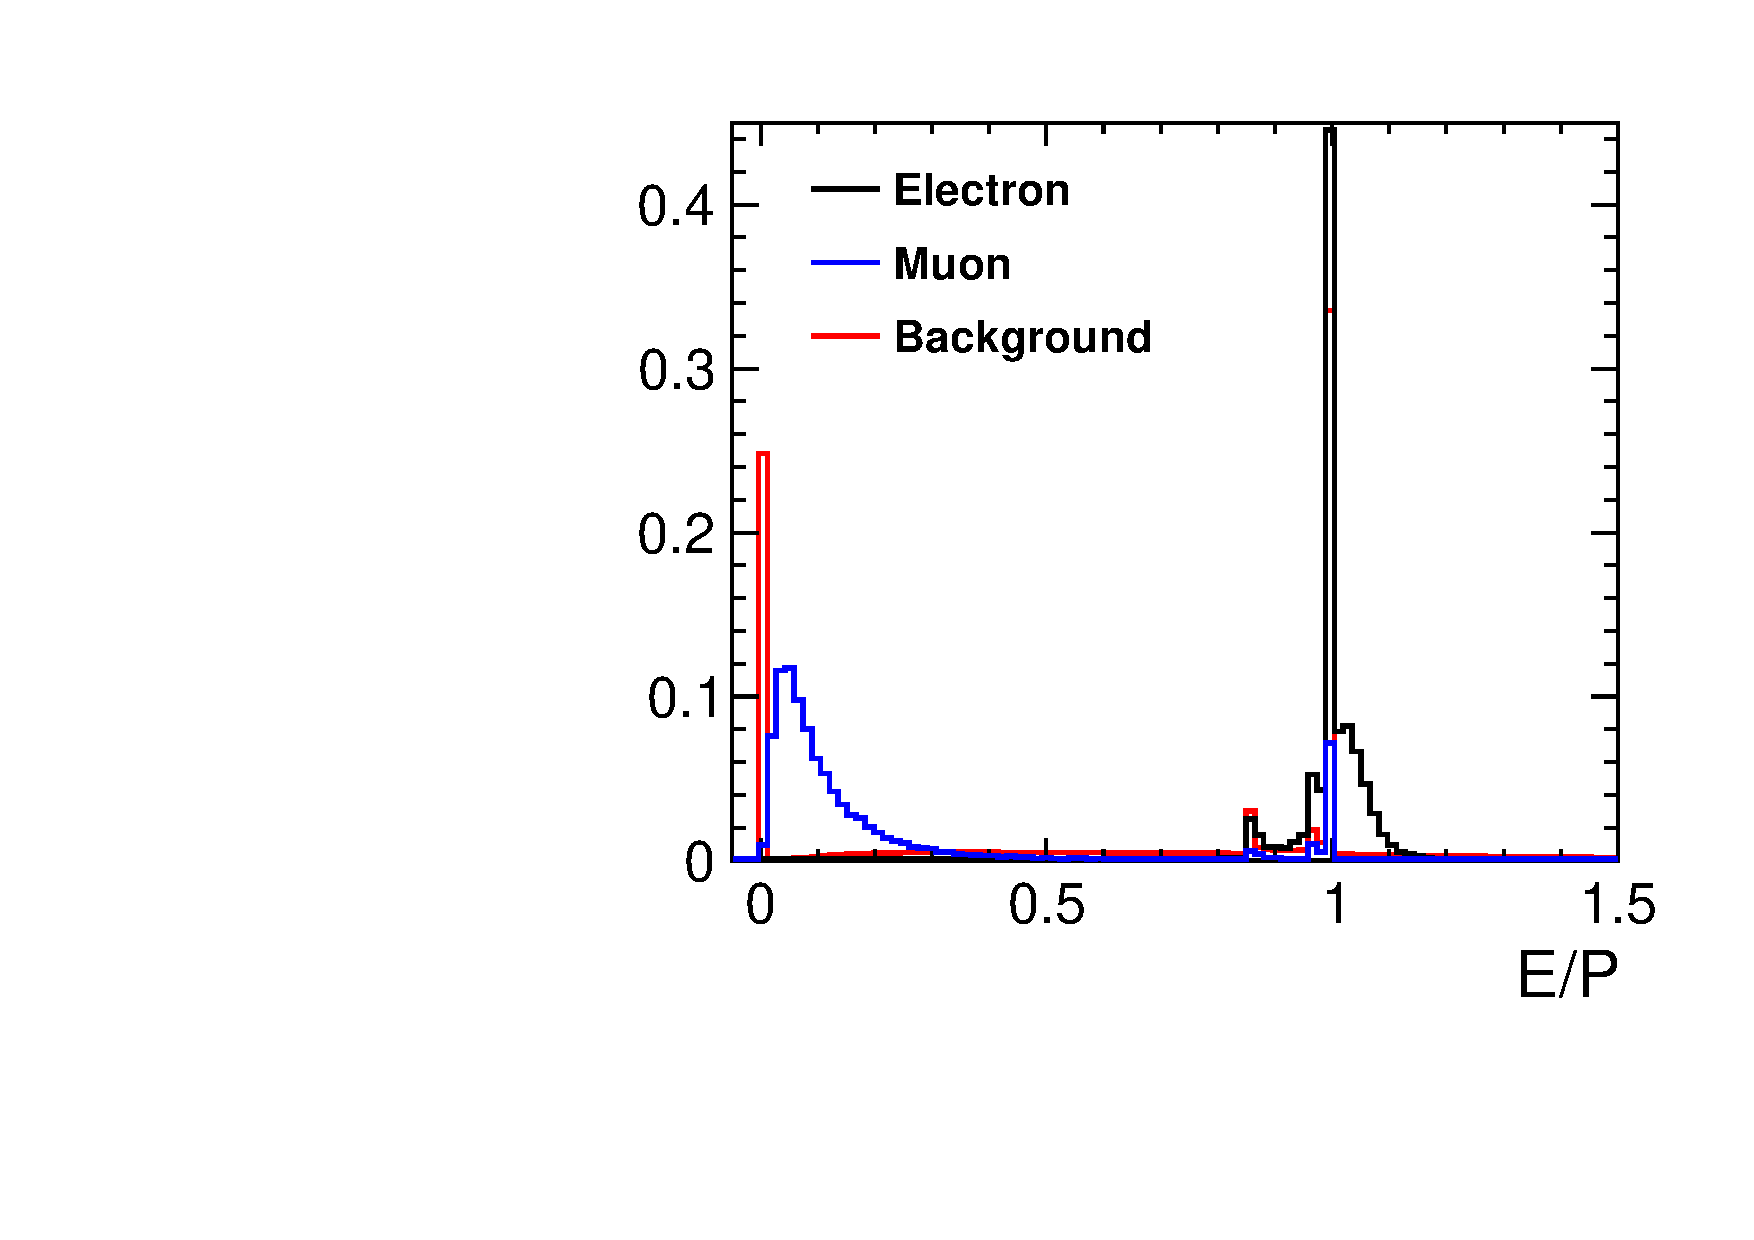
\includegraphics[width=1.0\linewidth,keepaspectratio]{HiggsAnalysis/figures/EByP}
    \caption{Ratio of the sum of the energy deposited in ECAL and HCAL to the momentum of the charged particle.}
  \end{subfigure}~
    \vspace{4ex}
  \begin{subfigure}[t]{.48\textwidth}
    \centering
    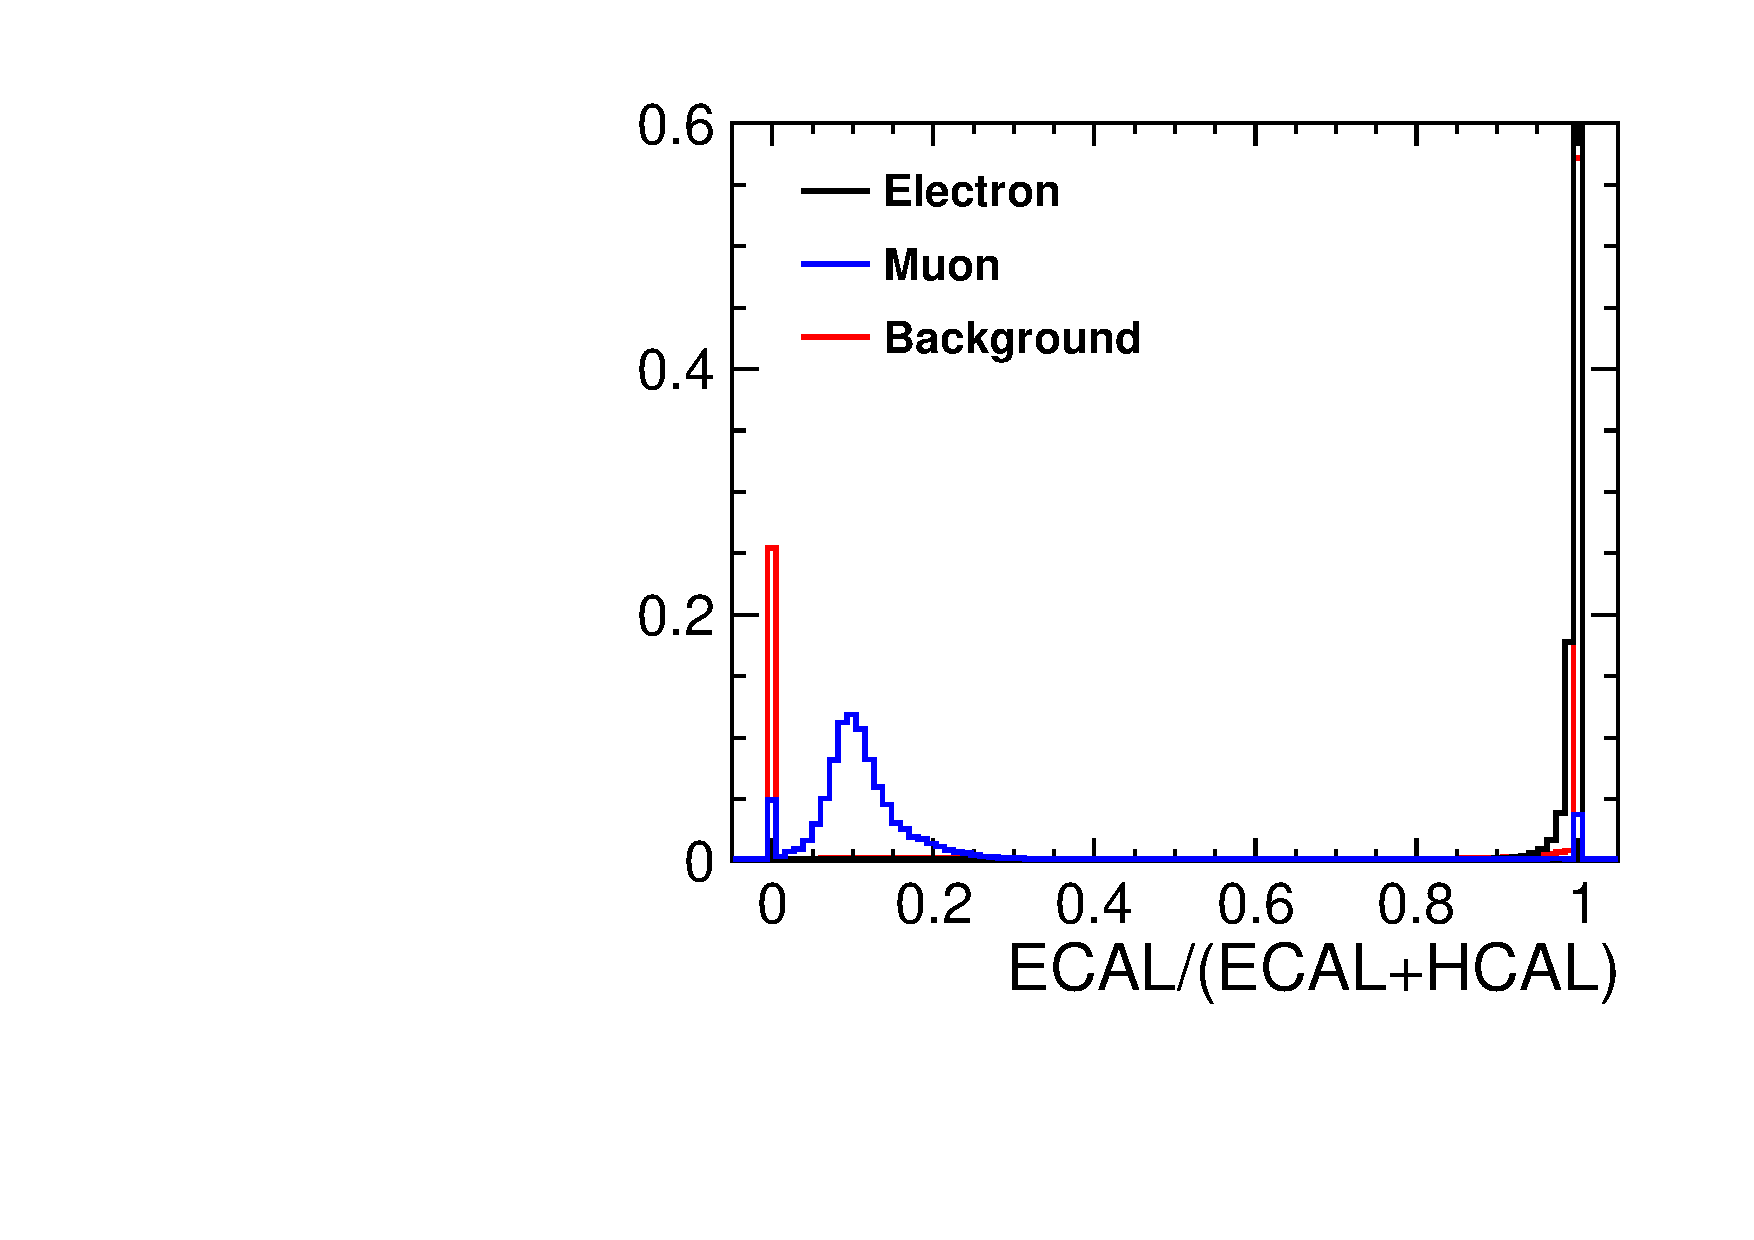
\includegraphics[width=1.0\linewidth,keepaspectratio]{HiggsAnalysis/figures/ECALByE}
    \caption{Ratio of the energy deposited in the ECAL to the total energy deposited in the calorimeters. }
  \end{subfigure}
  \caption[Parameters used for loose lepton selection]{Properties used for the loose lepton selection.  Note that in both cases, electrons and muons not produced in the initial W decay are considered as background.}
  \label{fig:lepfinding}
\end{figure}

The second method used a series of cuts to select the isolated lepton. The first stage of this was to group the particles in the event into four jets. This was done using the kt-algorithm with the E-scheme for recombination and an R-parameter of 0.4, as implemented in the FastJet package\cite{Cacciari:2011ma}. We then required that the energy of the isolated lepton (electron or muon) constituted more than 35\% of the visible energy of the jet within which it was contained. For electrons it was then required that at least 90\% of the total energy of the particle was deposited in the ECAL, and the ratio of energy to momentum for the particle was between 0.75 and 1.25. For muons it was required that less than 35\% of the total energy of the particle was deposited in the ECAL, and the ratio of energy to momentum should be between 0.01 and 0.60. The relevant distributions for these variables are shown in \reffig{fig:lepfinding}. This method yielded an efficiency of 91\% and a purity 74\%. Due to the lower purity of this method, leptons selected by this method are referred to as ``loose selected''. Although this approach is not as performant as the first method, it allows more than one lepton to be selected. As a result it is useful for discriminating between signal and background processes (e.g. $e^+e^-\rightarrow ZZ\rightarrow qqll$) as requirements can be placed on the number of leptons identified by this selection.

In summary, the first method is used to select a single isolated lepton, which is then used for reconstruction, while the number of lepton candidates selected by the second method is used as a discriminating variable to distinguish between signal and background processes. 

\subsection{Jet Finding}
\label{higgsjetfinding}

\begin{figure}
  \centering
  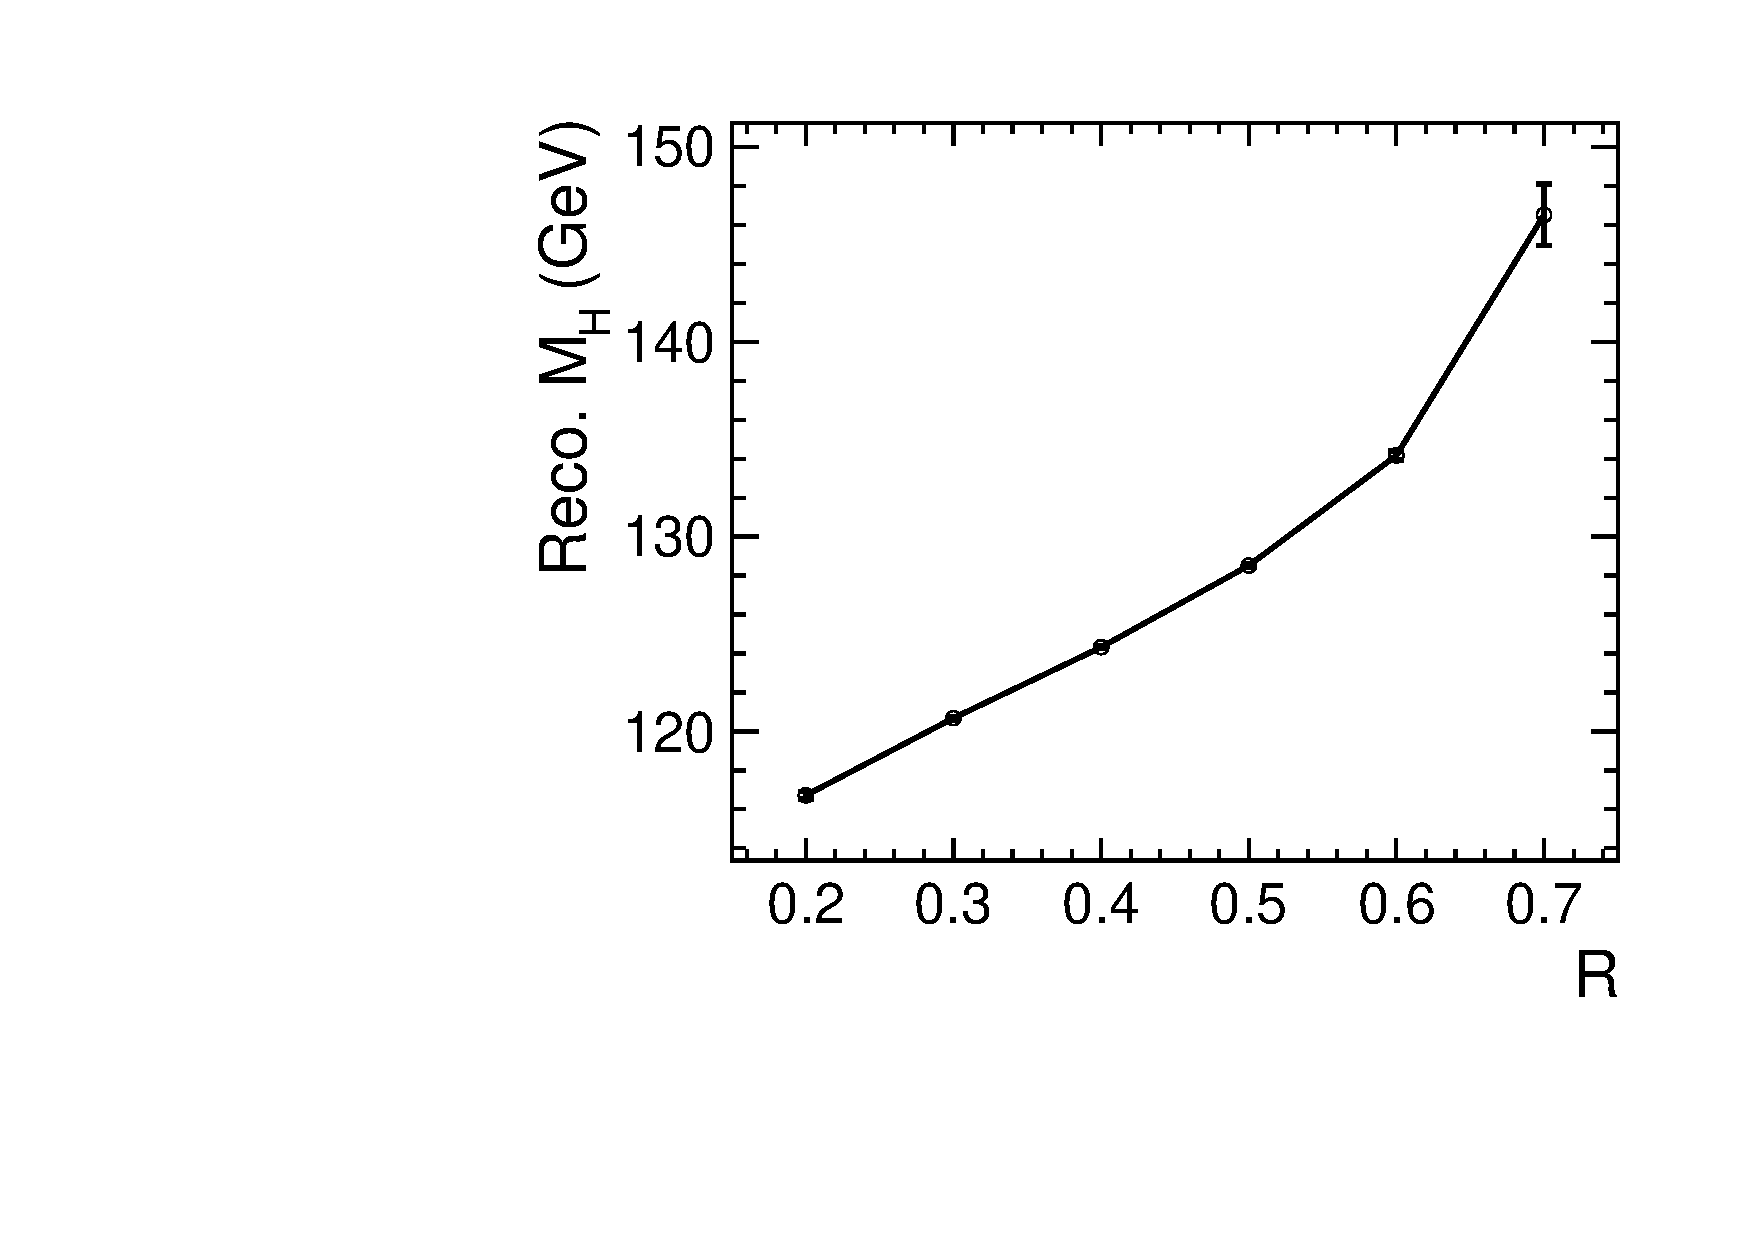
\includegraphics[width=0.7\textwidth,keepaspectratio]{HiggsAnalysis/figures/HiggsJetOptimization.pdf}
  \caption[Jet Reconstruction Optimization]{Reconstructed Higgs mass as a function of the jet radius parameter; reconstructed PFOs were used throughout except for the neutrino where MC truth information was used.}
  \label{fig:jetoptimization}
\end{figure}

\begin{figure}
  \centering
  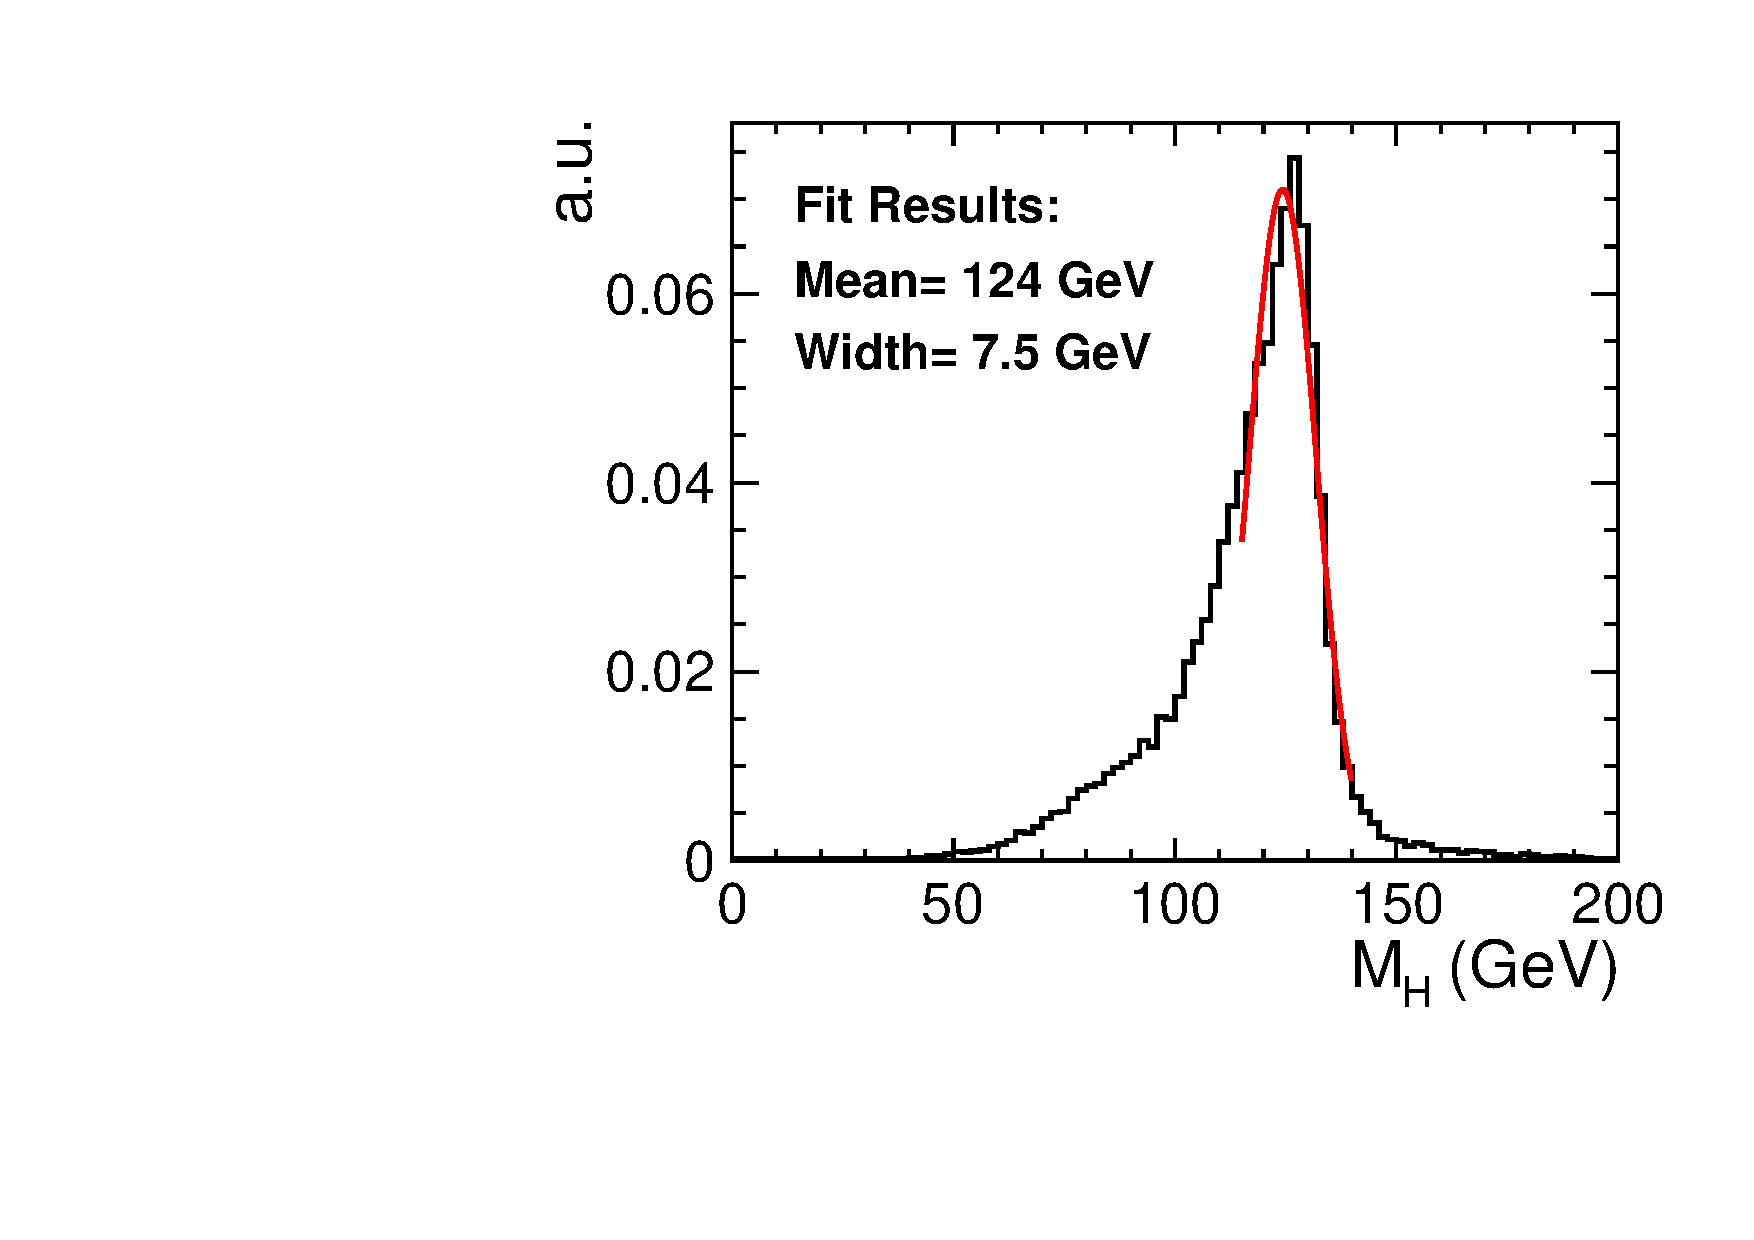
\includegraphics[width=0.7\textwidth,keepaspectratio]{HiggsAnalysis/figures/CheatHiggs04}
  \caption[Reconstructed Higgs Mass For Optimum Jet Radius]{Reconstructed Higgs mass for a jet radius of R=0.4; reconstructed PFOs were used throughout except for the neutrino where MC truth information was used.}
  \label{fig:cheatHiggsMass}
\end{figure}

\begin{figure}
  \centering
  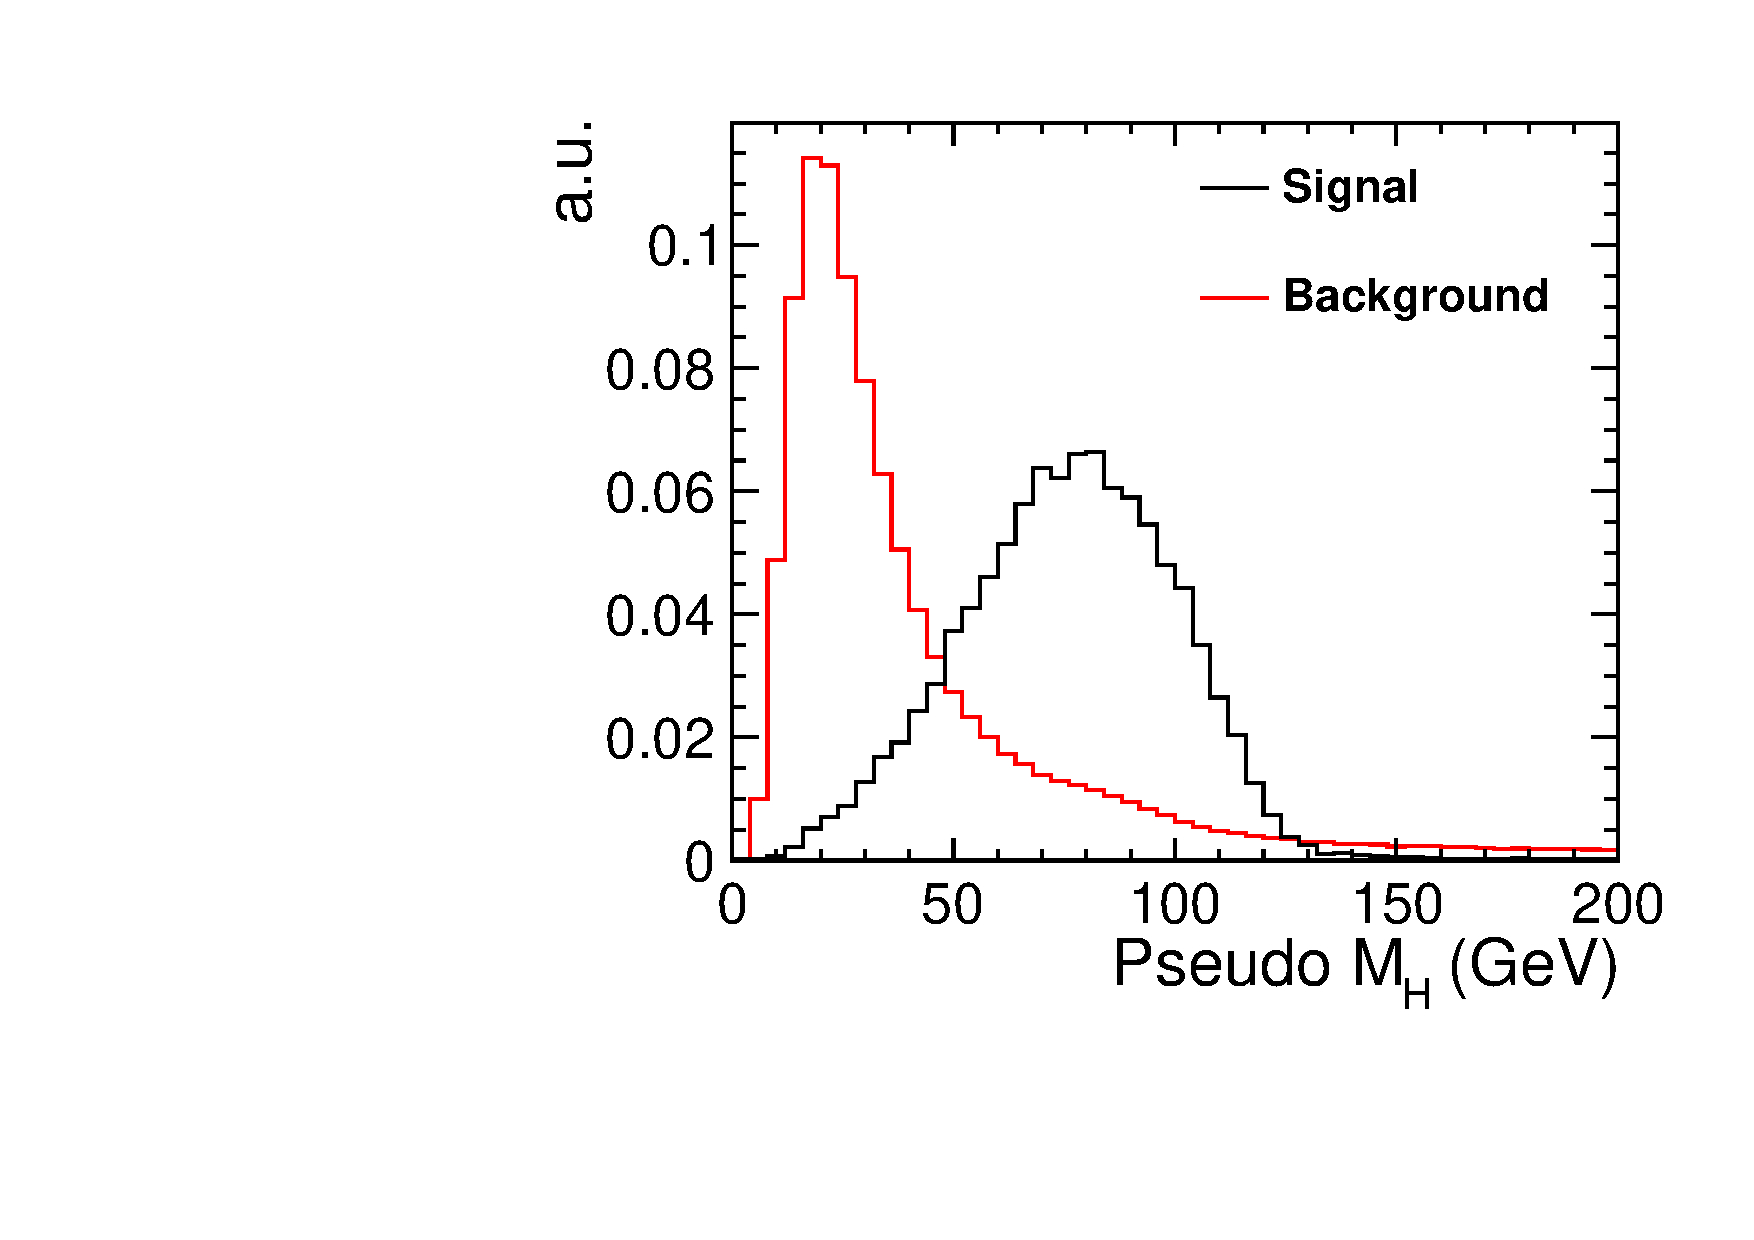
\includegraphics[width=0.7\textwidth,keepaspectratio]{HiggsAnalysis/figures/PseudoHiggs.pdf}
  \caption[Reconstructed Higgs Mass]{Reconstructed invariant mass of the lepton + quark pair system for signal events and the combined total background when using a jet radius of R=0.4. Both samples are normalised to unity.}
  \label{fig:pseudoHiggsMass}
\end{figure}


Following the lepton finding, the remaining PFOs (excluding the isolated charged lepton) are forced into two jets to reconstruct the properties of the two quarks produced from the hadronic W decay. This was carried out using the exclusive kt algorithm as implemented in FastJet. This is a sequential jet finding algorithm and follows the following procedure:

\begin{enumerate}
\item For each particle calculate its distance from the beam:
\begin{center}
  $d_{iB} = p_{Ti}^2$
\end{center}
\item For every pair of particles calculate the distance between them:
\begin{center}
  $d_{ij}=min(p_{Ti}^2,p_{Tj}^2)\Delta R_{ij}^2/R^2$
\end{center}
where $\Delta R_{ij}^2=(y_i-y_j)^2 + (\phi_i-\phi_j)^2$, $i$ and $j$ label particles, $p_T$ is transverse momentum, $y$ is rapidity, $\phi$ is azimuthal angle and $R$ is a tuneable parameter referred to as the jet radius.
\item Find the minimum of all the $d_{ij}$ and $d_{iB}$. If this corresponds to a $d_{ij}$ then merge particles $i$ and $j$ by summing their four-momenta. If it corresponds to a $d_{iB}$ then declare particle i to be part of the beam and remove it.
\item Repeats steps 1)-3) until there are only the desired number of jets remaining
\end{enumerate}

The optimization of the $R$ parameter was performed using Monte Carlo information to determine what mass would be measured for the reconstructed Higgs for various values of R, when including the Monte Carlo truth kinematic information of the lepton neutrino in the reconstruction. The results of this optimization study are shown in \reffig{fig:jetoptimization}. The minimal bias in the reconstructed mass was found for an R value of 0.4, indicating successfull reconstruction of the quark pair. It is possible a smaller bias could be found by tuning the R parameter to multiple decimal places however given the separation seenbetween signal and background processes for R=0.4 seen in \reffig{fig:pseudoHiggsMass} this is not believed to be necessary. The resulting Higgs mass distribution is shown in \reffig{fig:cheatHiggsMass}. Note that this mass is only used for optimization of the jet reconstruction. It is never used for the event selection as it is not possible to calculate this mass without using MC truth information. For event selection, the pseudo Higgs mass corresponding to the invariant mass of the lepton and quark pair system is used instead. This is shown in \reffig{fig:pseudoHiggsMass}.



\section{Flavour Tagging}

\begin{figure}
  \centering
  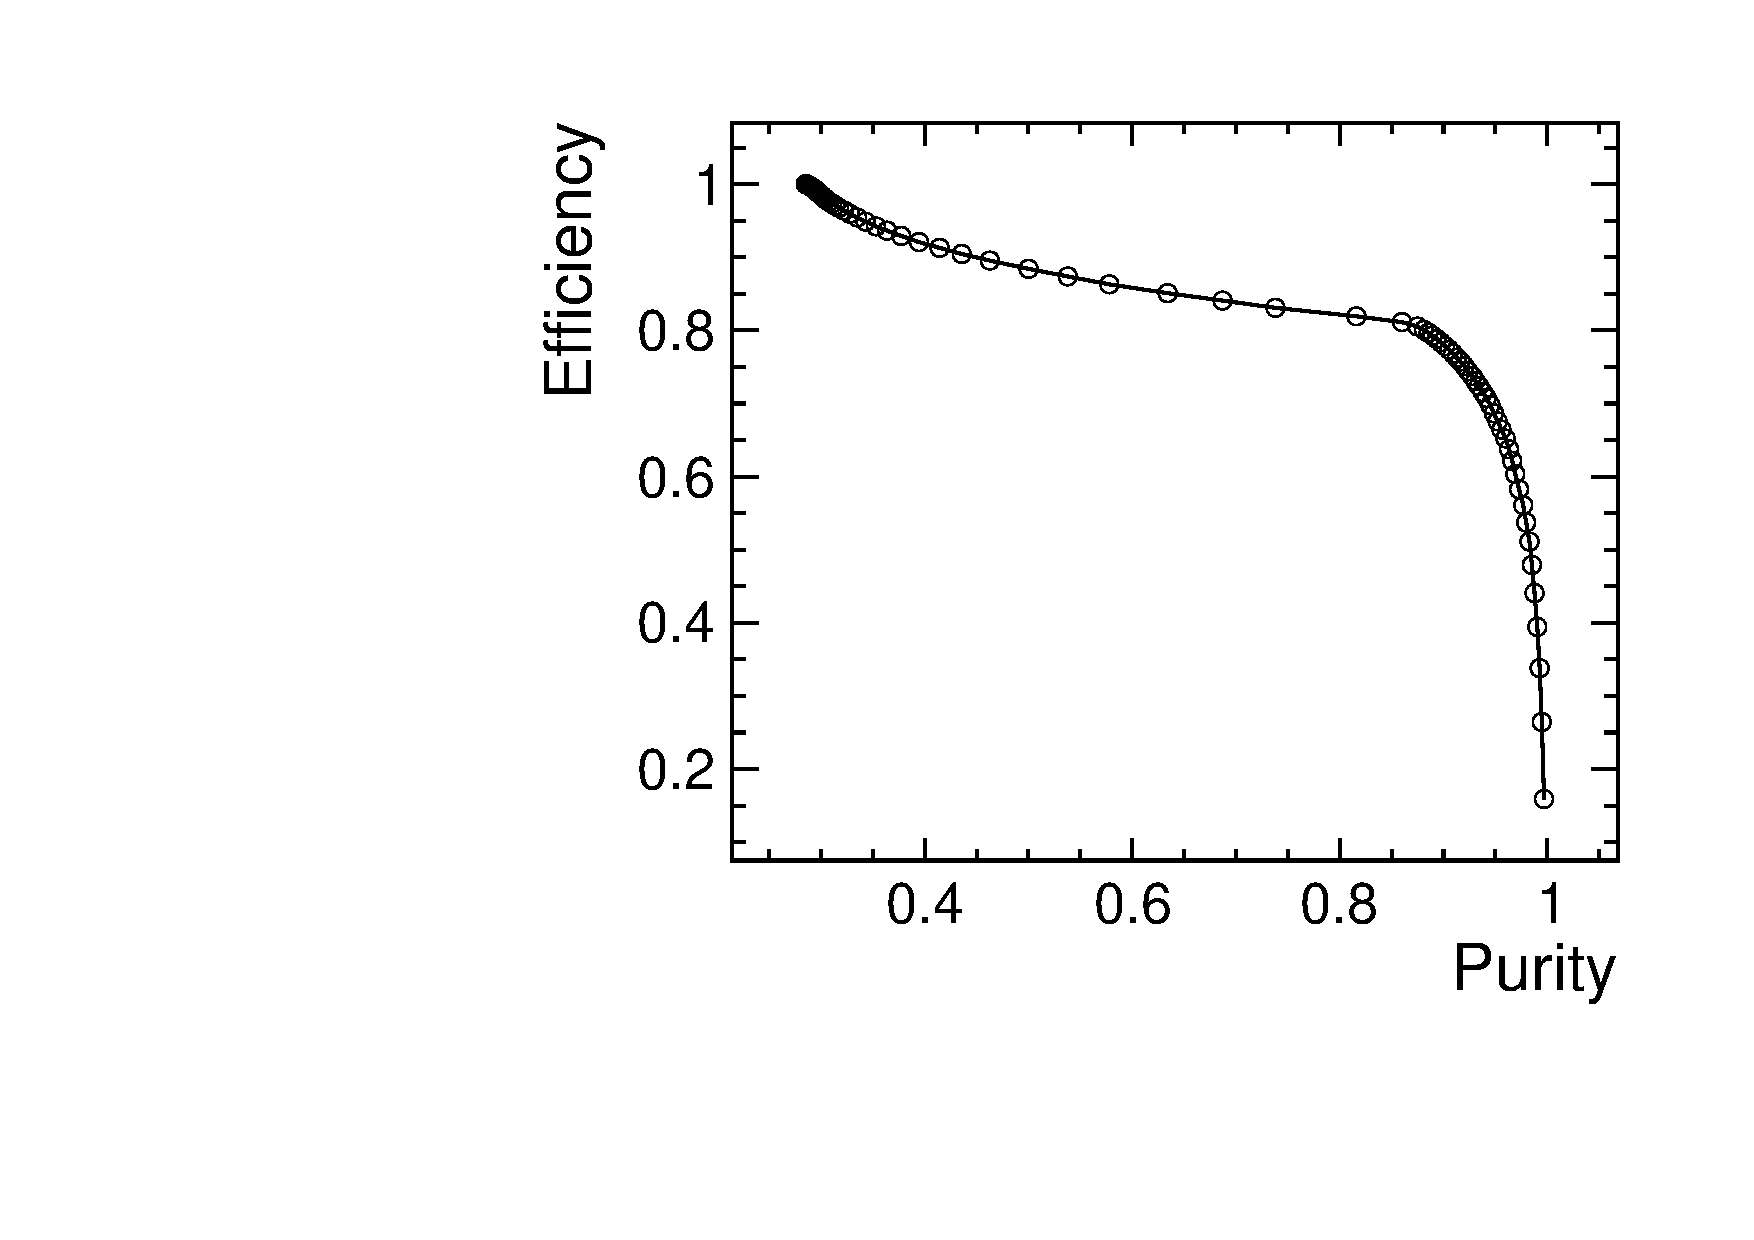
\includegraphics[width=0.78\textwidth,keepaspectratio]{HiggsAnalysis/figures/updatedpurityvsefficiency.pdf}
  \caption[B-Tagging Purity vs Efficiency]{Purity vs efficiency for identifying b-jets, obtained from a sample of Z$\rightarrow$ light, c and b quark events simulated at $\sqrt{s}=$1.4TeV.}
  \label{btag}
\end{figure}

Flavour tagging of events was performed using LCFIPlus v00-05-02 \cite{Suehara:2015ura}. Three neural nets were used to identify u/d/s, b and c quarks with training for each of these based on samples of 50,000 simulated ee$\rightarrow$ Z$\nu\nu$, Z$\rightarrow$qq 1.4~TeV events. The neural nets are trained on a variety of parameters such as impact parameters, vertex masses, track multiplicity and  track lengths. Application of these neural nets returned two parameters for jets within the event that quantify the probability of the jet being either a b-jet or c-jet. For this analysis, identifying b-jets is more useful for discriminating against the relevant backgrounds. Performance of the b-tagging was evaluated by applying the neural nets to a sample of 150,000 events containing an equal number of Z$\rightarrow$ light, c and b quarks. It can be seen from \reffig{btag} that a purity of 90\% can be achieved while still retaining an efficiency of 80\%, where efficiency is defined as the fraction of true b-jets that pass the b-tag selection, and purity is defined as the fraction of all jets that pass the b-tag that came from true b-jets.

\section{Event Selection}

Event selection was performed in two steps. The first of these is referred to as the preselection and removes easily identifiable backgrounds with minimal loss of signal events by applying loose cuts. The cuts used were as follows:

\begin{enumerate}

\item Mass of the reconstructed Higgs $<$ 200 GeV
\item At least one loose selected lepton in the event
\item Missing energy of the event must lie in the range 800--1350 GeV
\item Energy of the hadronically decaying W $<$ 600 GeV

\end{enumerate}


\begin{figure}
  \centering
  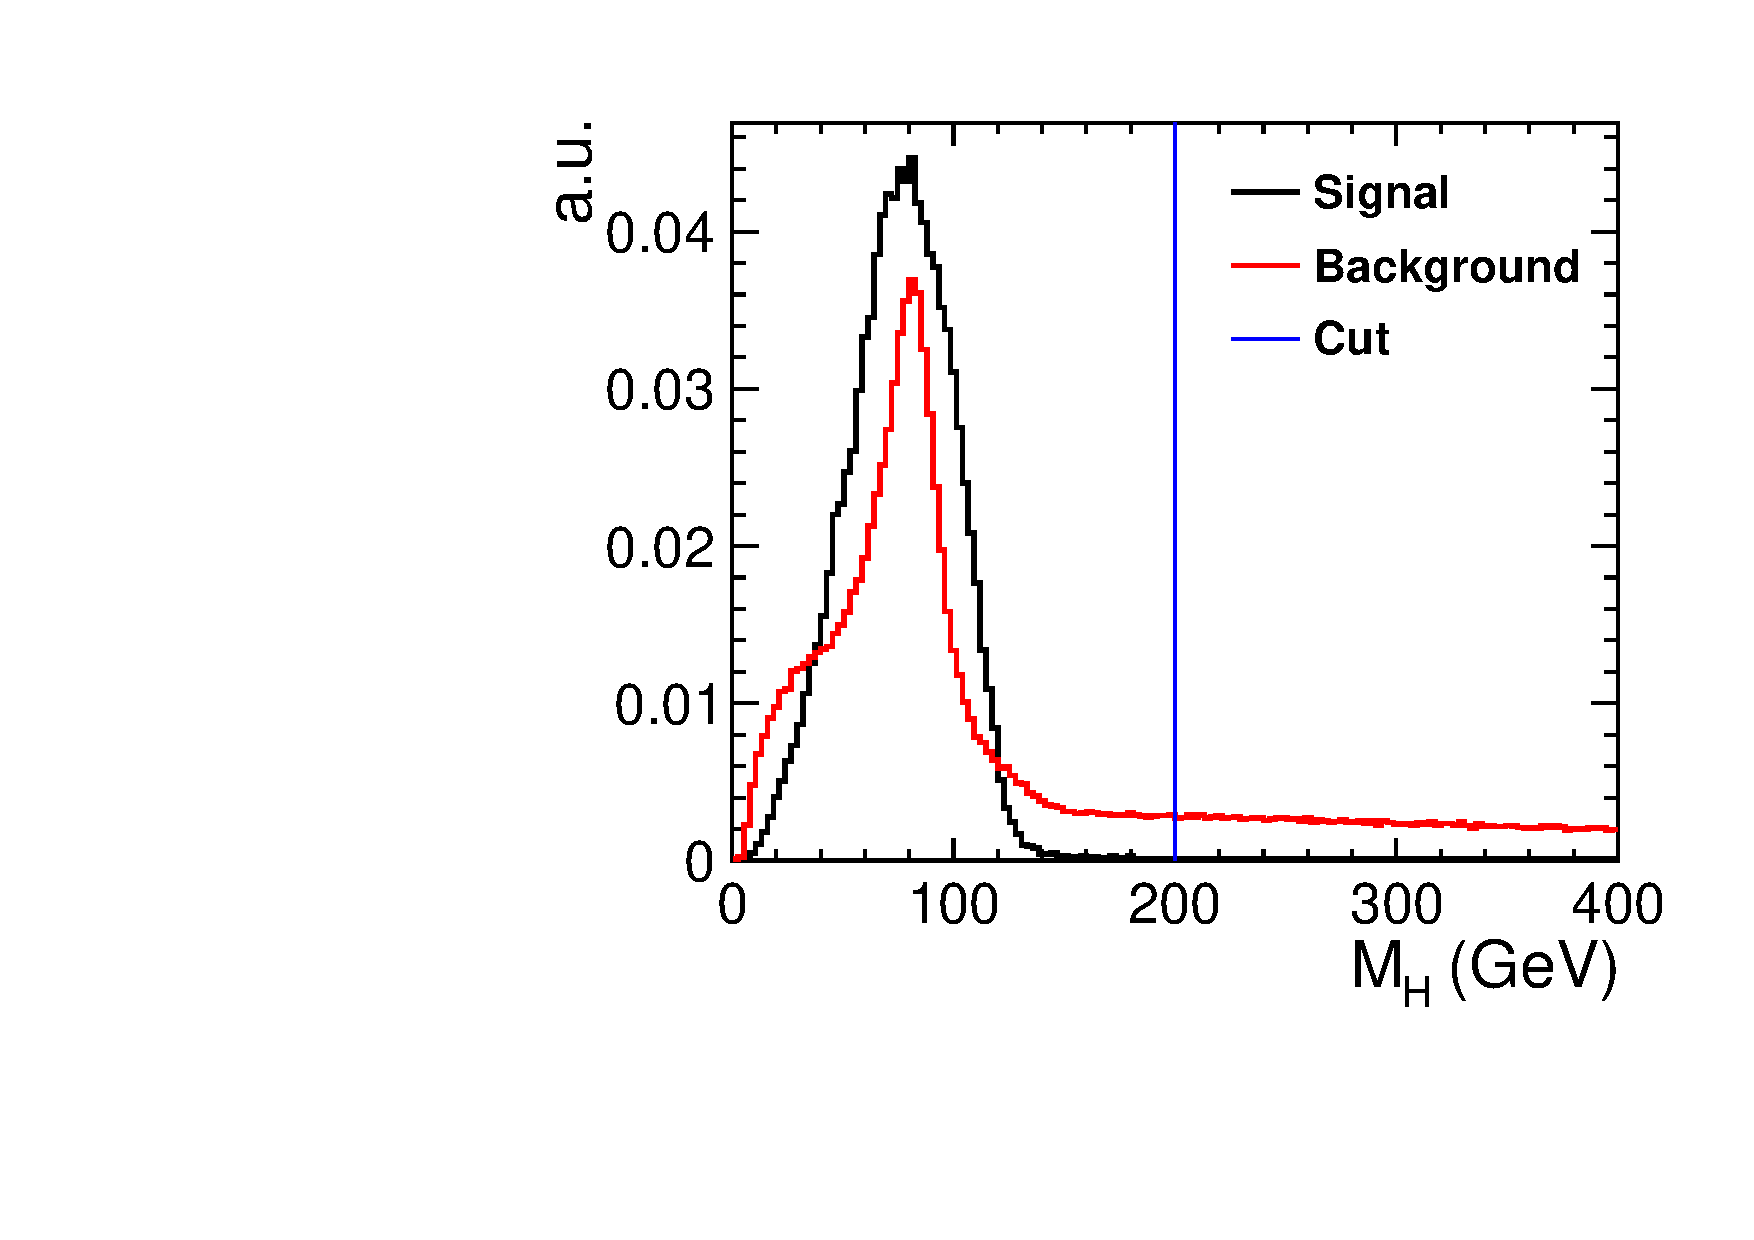
\includegraphics[width=0.78\textwidth,keepaspectratio]{HiggsAnalysis/figures/PseudoHiggs_PreSelection}
  \caption[Reconstructed Higgs mass for signal and background events]{Mass of the reconstructed Higgs for the signal process and dominant backgrounds ($ee\rightarrow H\nu\nu$ (non-signal) and $ee\rightarrow qql\nu$). Both signal and background are normalised to unity.}
  \label{fig:HMassPreSel}
\end{figure}

\begin{figure}
  \centering
    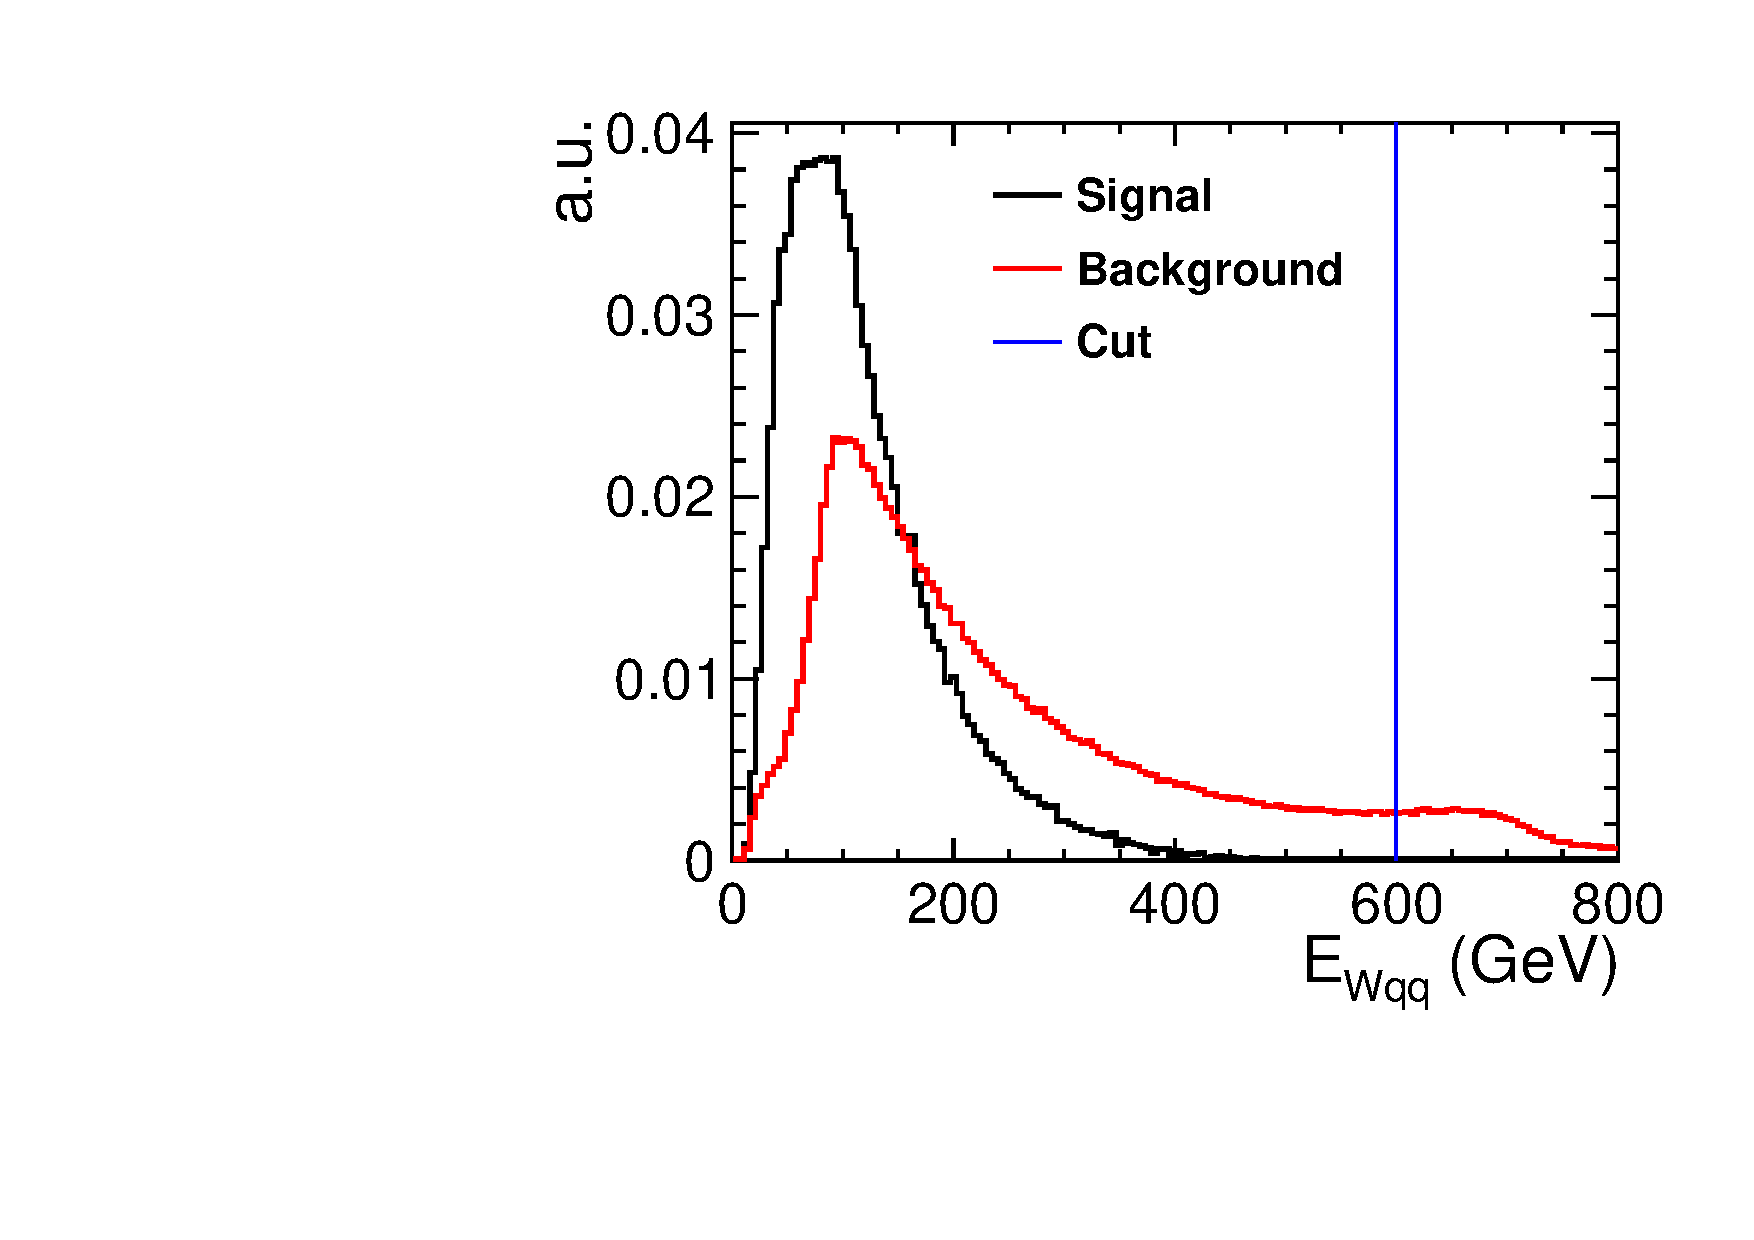
\includegraphics[width=0.78\linewidth,keepaspectratio]{HiggsAnalysis/figures/EWqq_PreSelection}
    \caption[Energy of the hadronically decaying W Boson for signal and background events]{Energy of the hadronically decaying W Boson for the signal process and dominant backgrounds ($ee\rightarrow H\nu\nu$ (non-signal) and $ee\rightarrow qql\nu$). Both signal and background are normalised to unity.}
  \label{fig:WPreSel}
\end{figure}

\begin{figure}
  \centering
  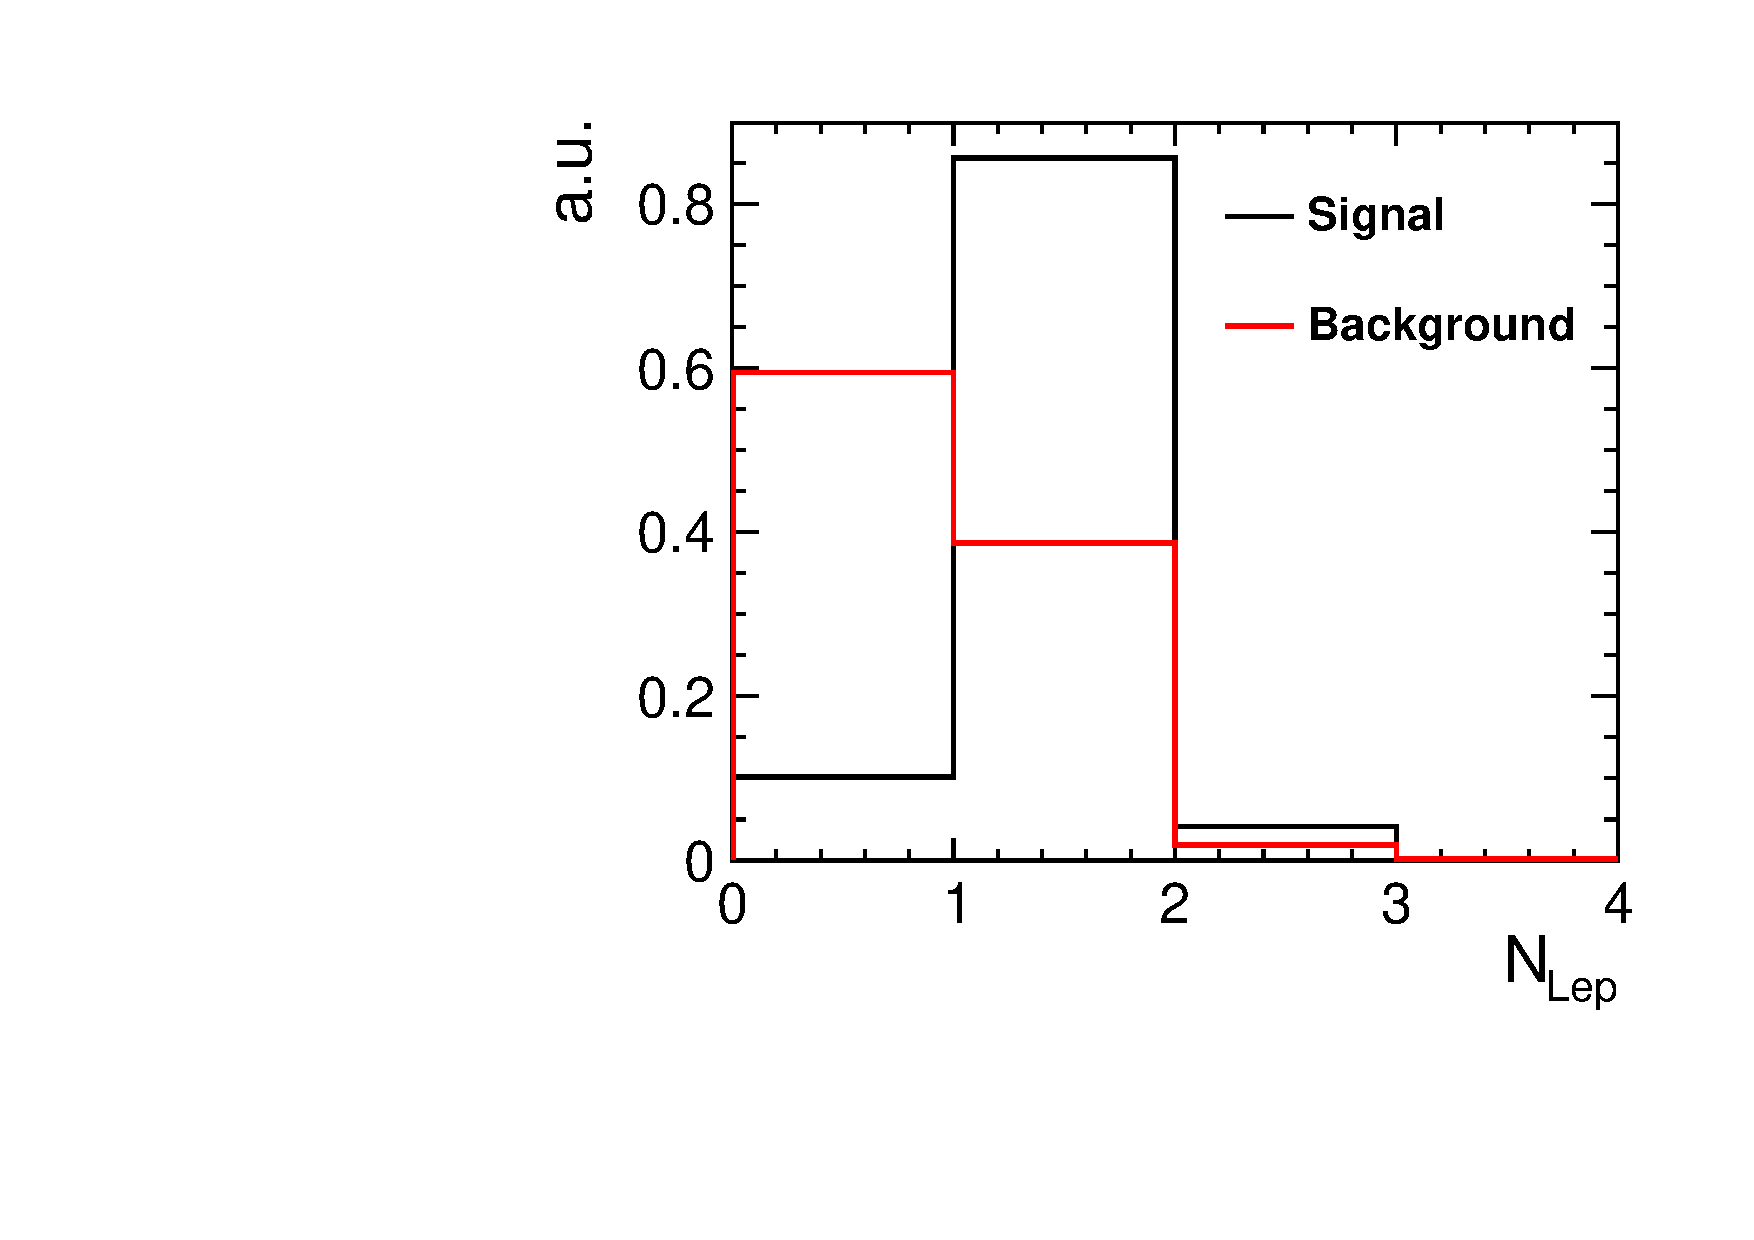
\includegraphics[width=0.78\textwidth,keepaspectratio]{HiggsAnalysis/figures/nLep_PreSelection}
  \caption[Number of reconstructed loose selected lepton for signal and background events]{Number of loose selected leptons for the signal process and dominant backgrounds ($ee\rightarrow H\nu\nu$ (non-signal) and $ee\rightarrow qql\nu$). Both signal and background are normalised to unity.}
  \label{fig:nLepPreSel}
\end{figure}

\begin{figure}
  \centering
  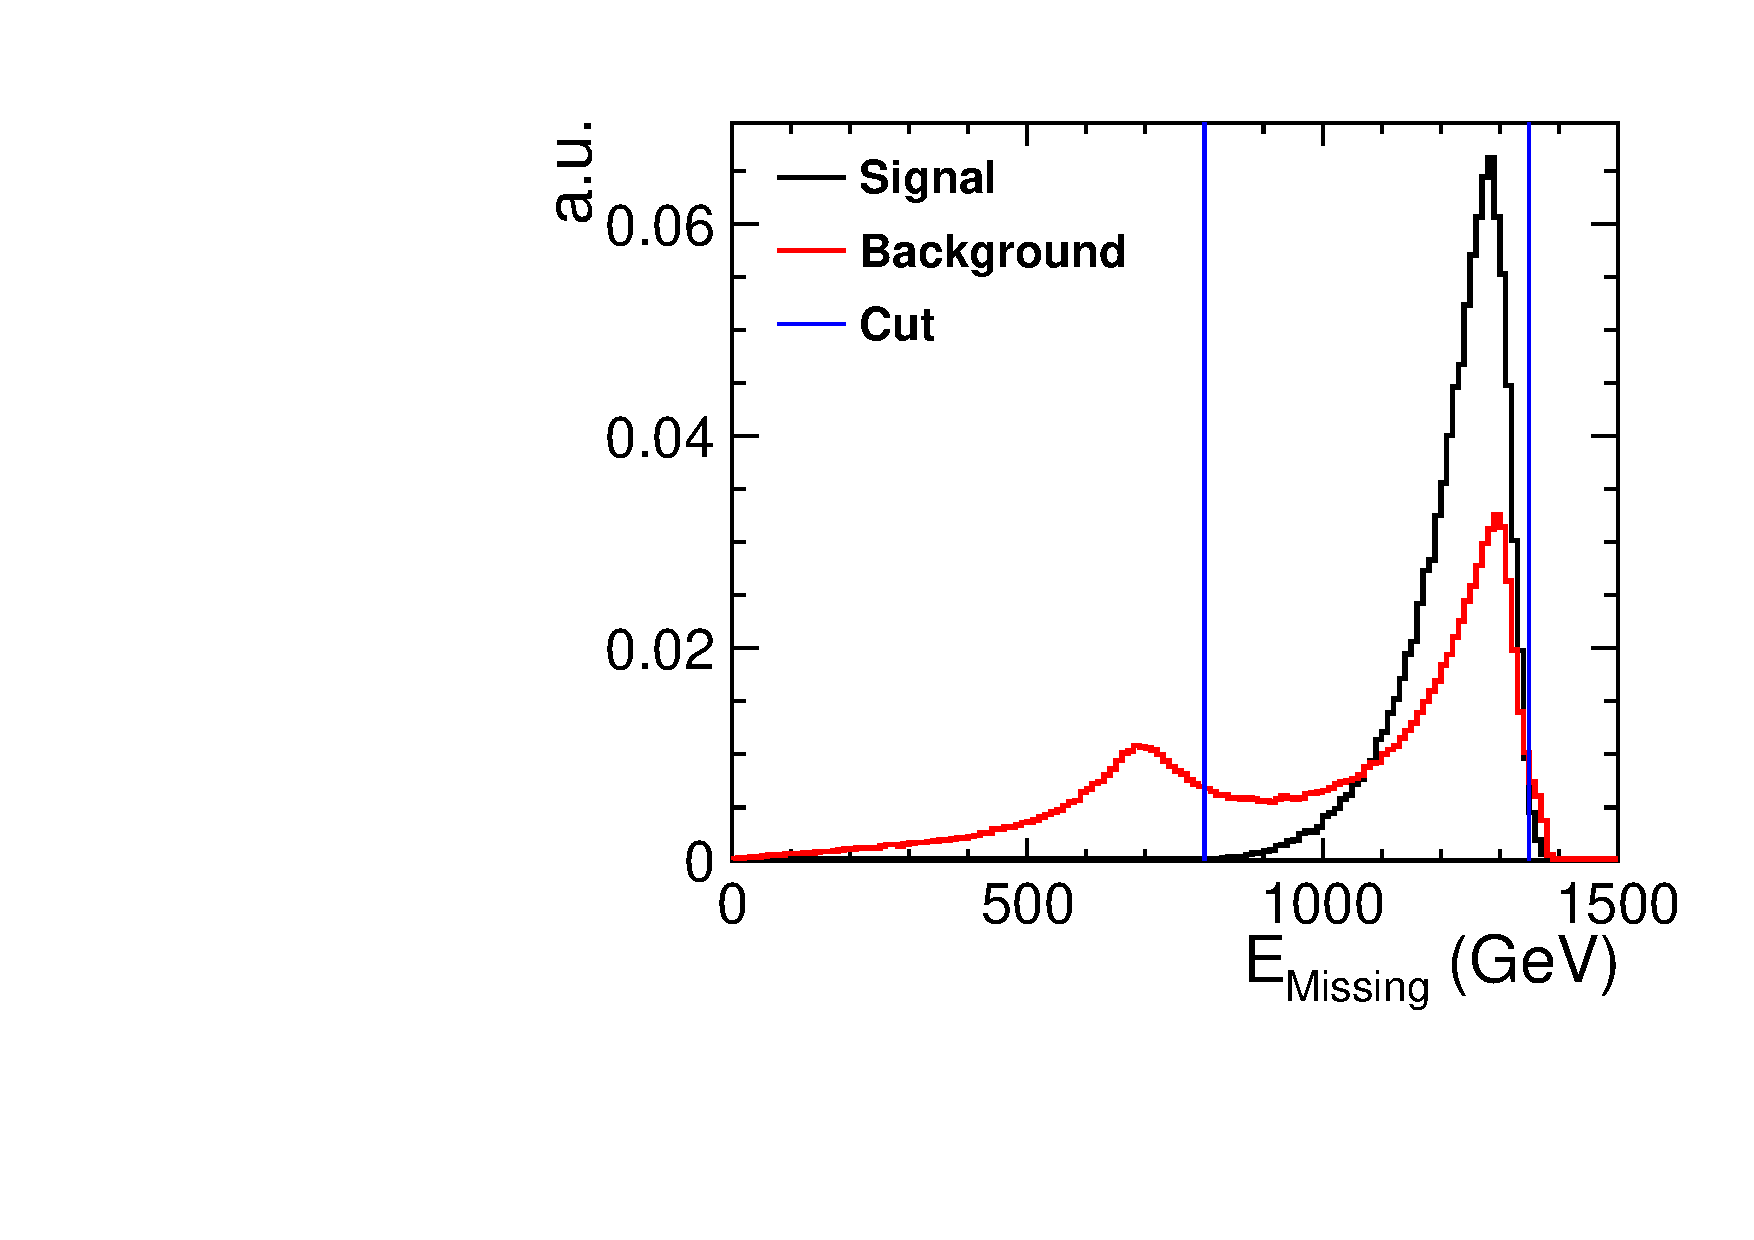
\includegraphics[width=0.78\textwidth,keepaspectratio]{HiggsAnalysis/figures/EMissing_PreSelection}
  \caption[Missing energy of signal and background events]{Missing energy for the signal process and dominant backgrounds ($ee\rightarrow H\nu\nu$ (non-signal) and $ee\rightarrow qql\nu$). The peak at $\sim$700~GeV is due to $ee\rightarrow qql\nu$ which has only one neutrino and thus less missing energy relative to the $ee\rightarrow H\nu\nu$ samples. Both signal and background are normalised to unity.}
  \label{fig:EMissPreSel}
\end{figure}

\begin{figure}
  \centering
  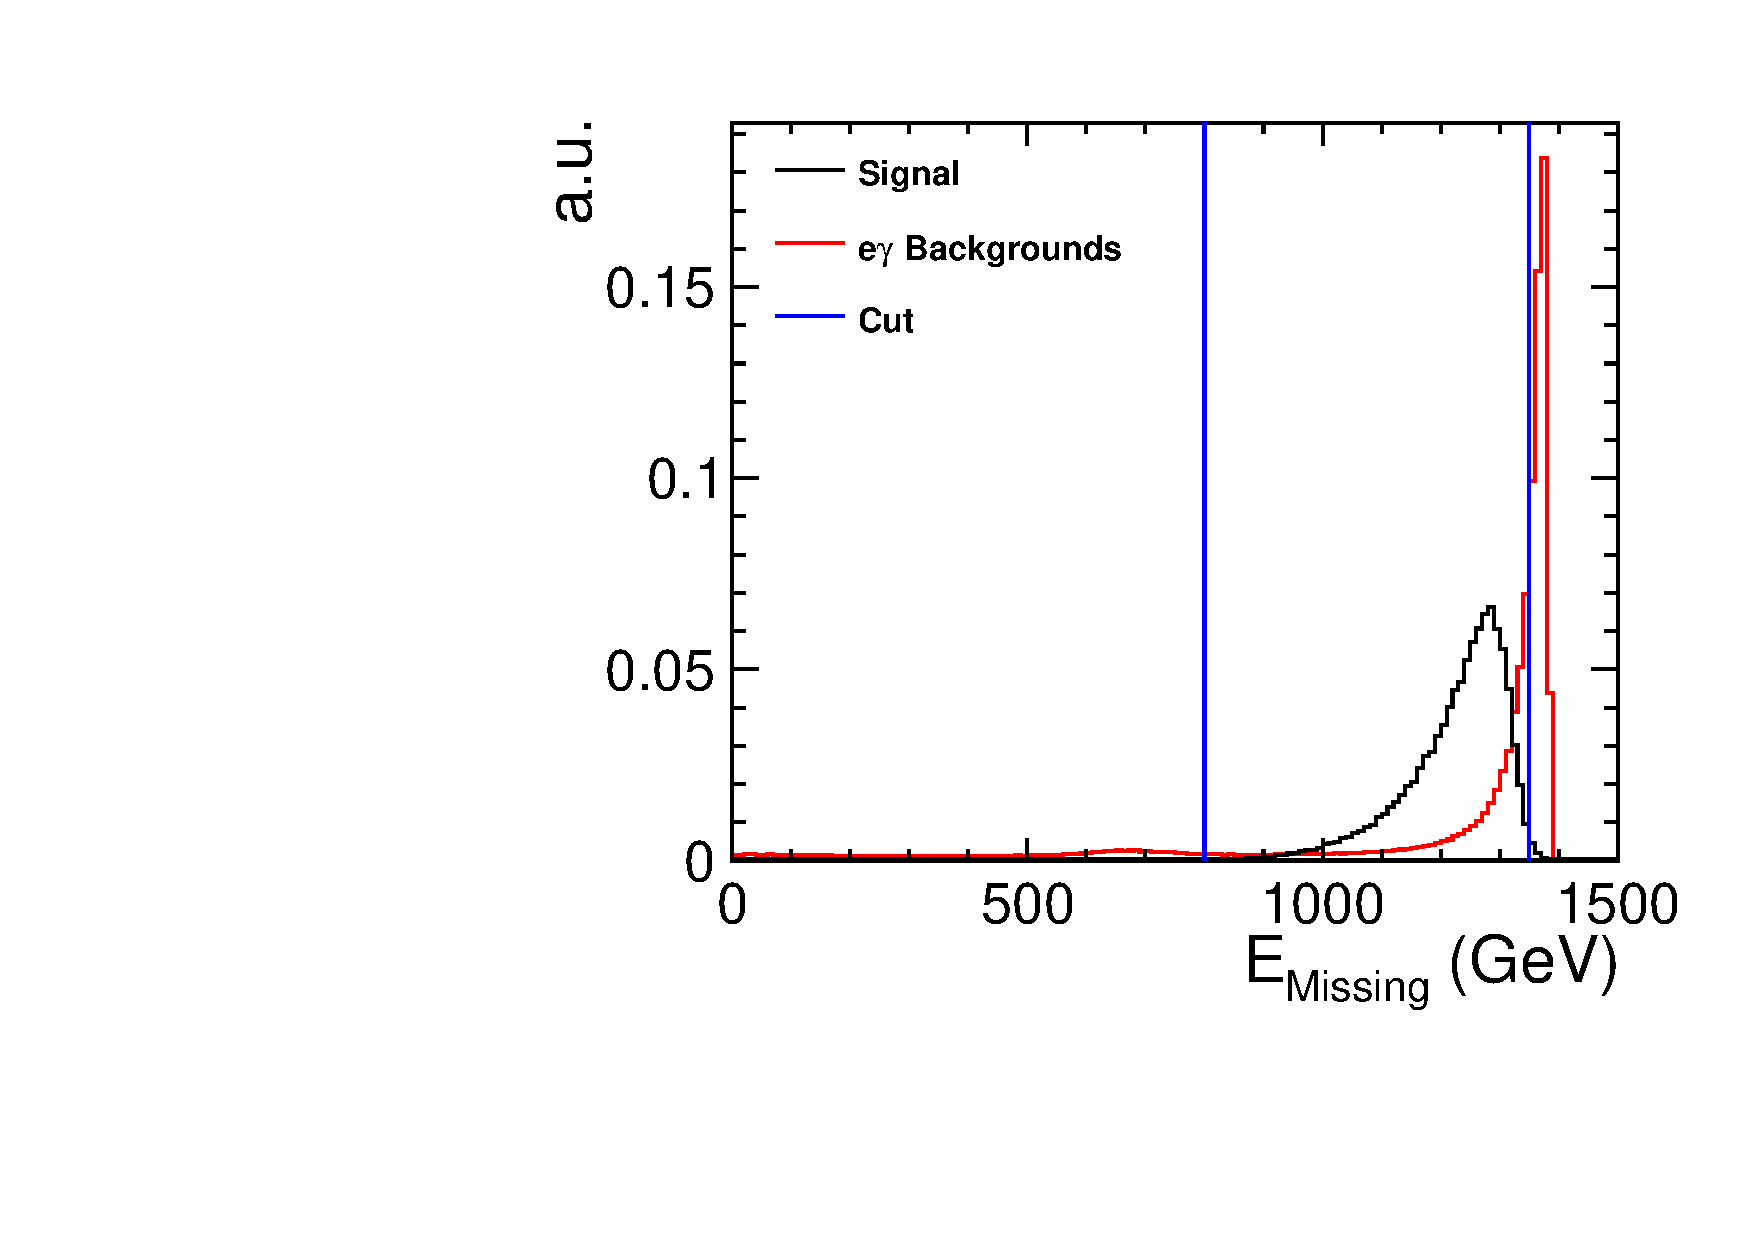
\includegraphics[width=0.78\textwidth,keepaspectratio]{HiggsAnalysis/figures/EMissing_PreSelection_alt}
  \caption[Missing energy of signal and e$\gamma$ events]{Missing energy for the signal process and e$\gamma$ backgrounds. Both signal and background are normalised to unity.}
  \label{fig:EMissPreSelAlt}
\end{figure}

\begin{figure}
  \centering
  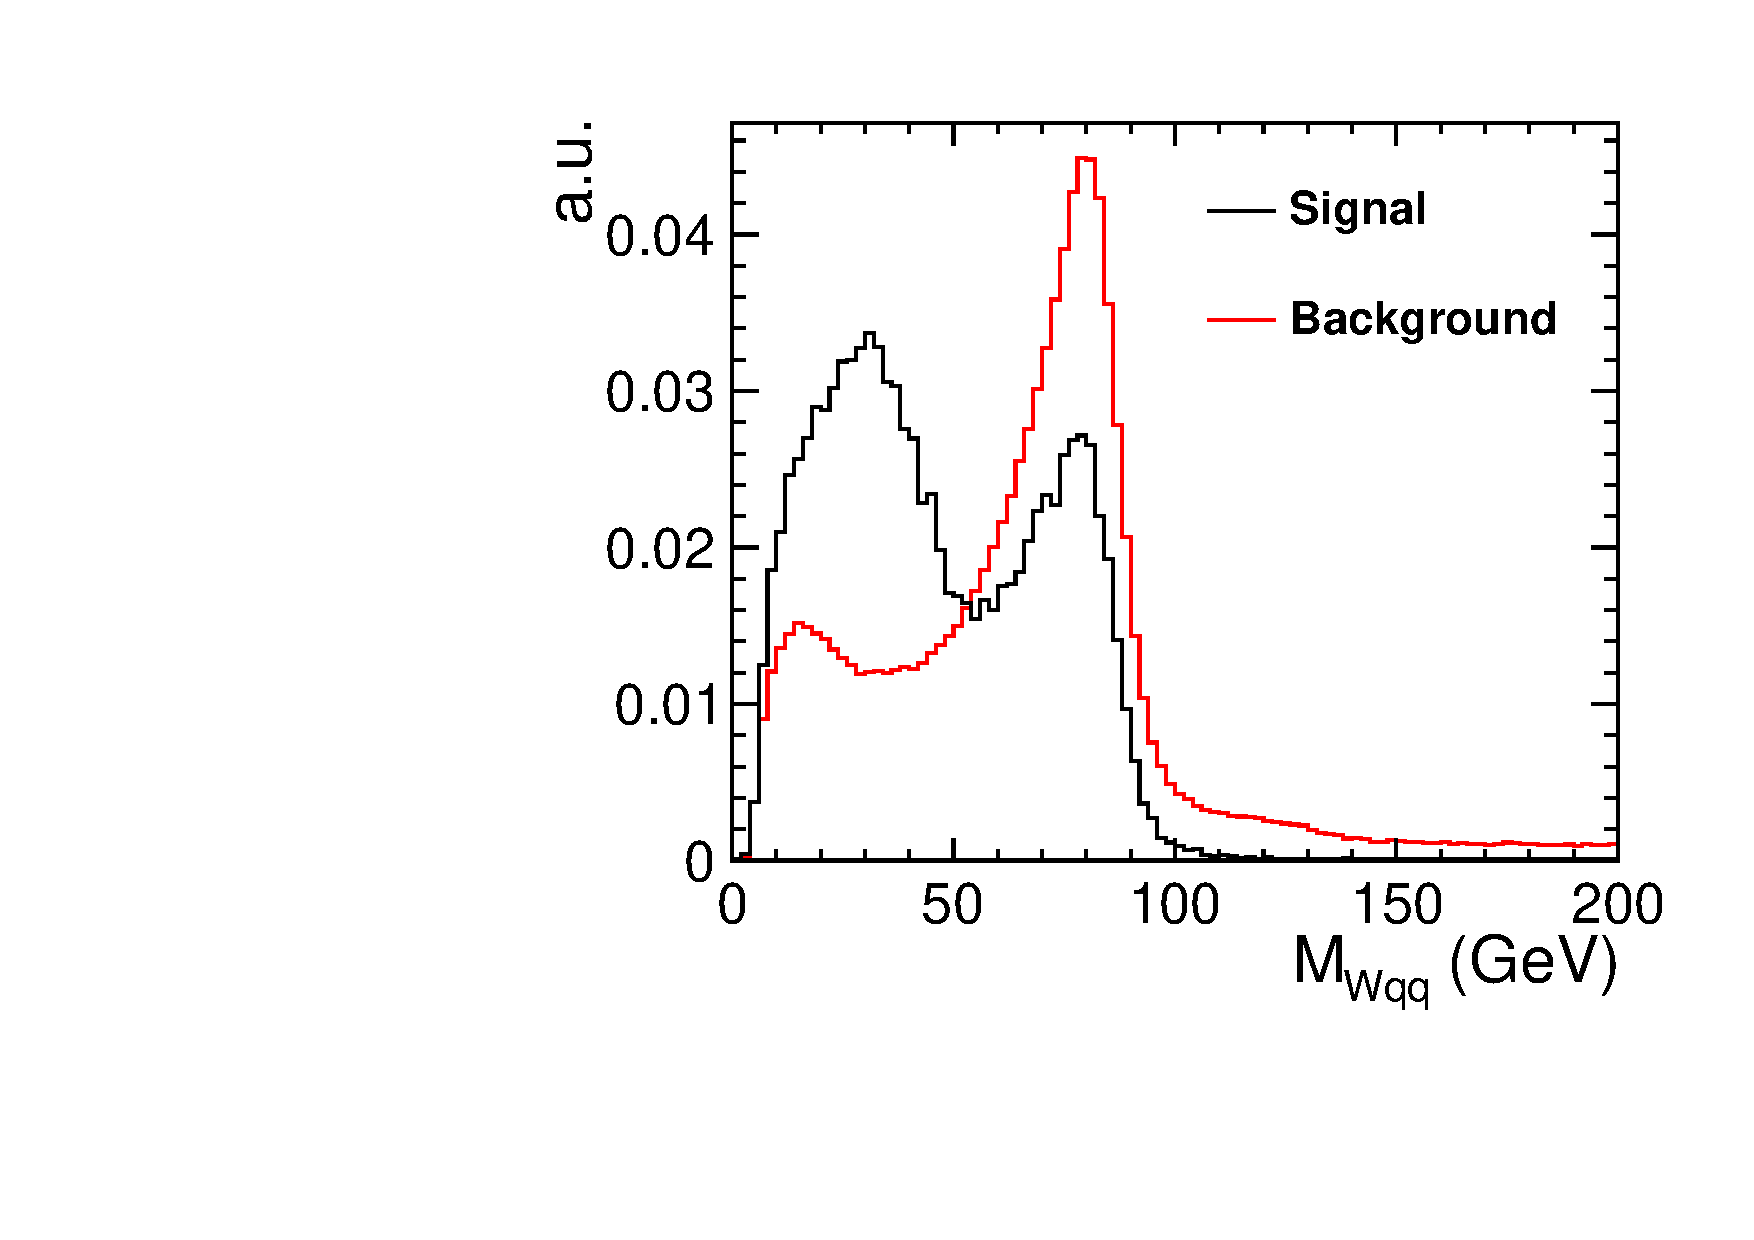
\includegraphics[width=0.78\textwidth,keepaspectratio]{HiggsAnalysis/figures/MWqq_PreSelection}
  \caption[Reconstructed W mass for signal and background events]{Reconstructed mass for the signal process and dominant backgrounds ($ee\rightarrow H\nu\nu$ (non-signal) and $ee\rightarrow qql\nu$). Both signal and background are normalised to unity.}
  \label{fig:WMass}
\end{figure}


With the exception of the upper limit placed on the missing energy, these cuts were optimised for the removal of the two dominant background processes ($ee\rightarrow H\nu\nu$ (non-signal) and $ee\rightarrow qql\nu$.) The upper limit on missing energy is instead designed to remove $e\gamma$ events which are typically collinear with the beam axis and so deposit minimal energy in the detector. This cut alone removes approximately half of all $e\gamma$ events. The distribution of the variables associated with these cuts before the preselection is applied are shown for the signal and dominant backgrounds($ee\rightarrow H\nu\nu$ (non-signal) and $ee\rightarrow qql\nu$) in \reffig{fig:HMassPreSel}--\ref{fig:EMissPreSelAlt} and the resulting efficiencies for the signal and background processes after the preselection criteria are applied are shown in \reftab{fig:preseleff}. Along with the cut on the mass of the Higgs candidate, one might naively expect a similar cut to be placed upon the mass of the reconstructed W. However, due to the relative masses of the Higgs and W the W's produced in the Higgs decay cannot always be on shell. In practice one finds that the kinematically favoured solution is that one W is produced on shell while the second is produced with a mass of $\sim$45 GeV. As a result, as can be seen in \reffig{fig:WMass}, it is challenging to separate background events from signal events in which the hadronically decaying W is produced off shell.

\begin{table}
  \centering
  \begin{tabular}{l r r }
   \toprule
    Process & Cross Section(fb) & Preselection Efficiency (\%)     \\
    \midrule
    Signal             & 17.3    &   89.3 \\ 
    \midrule
    ee$\rightarrow$ H(WW$^*\rightarrow$qqqq)$\nu\nu$  & 27.4    &  4.12  \\
    \midrule
    ee$\rightarrow$ H($\rightarrow$ Other)$\nu\nu$ & 199.4 & 26.4  \\
    \midrule
    ee$\rightarrow$qq               & 4009.5    &  7.21 \\ 
    \midrule
    ee$\rightarrow$qqqq               & 1328.1    &  2.09  \\ 
    \midrule
    e$\gamma$$\rightarrow$eqq ($\gamma$ from EPA)                 & 32308    & 7.32   \\ 
    \midrule
    $\gamma$e$\rightarrow$eqq ($\gamma$ from BS)               &  56043   &  8.02 \\ 
    \midrule
    ee$\rightarrow$qq$\nu\nu$               & 787.7    & 9.18  \\ 
    \midrule
    ee$\rightarrow$qqll               & 2725.8    &   13.6 \\ 
    \midrule
    ee$\rightarrow$qql$\nu$              & 4309.7    &  7.90  \\ 
    \bottomrule
  \end{tabular}
  \caption[Preselection efficiencies]{Preselection efficiencies}
  \label{fig:preseleff}
\end{table}



\subsection{Boosted Decision Trees}

\begin{figure}
  \centering
  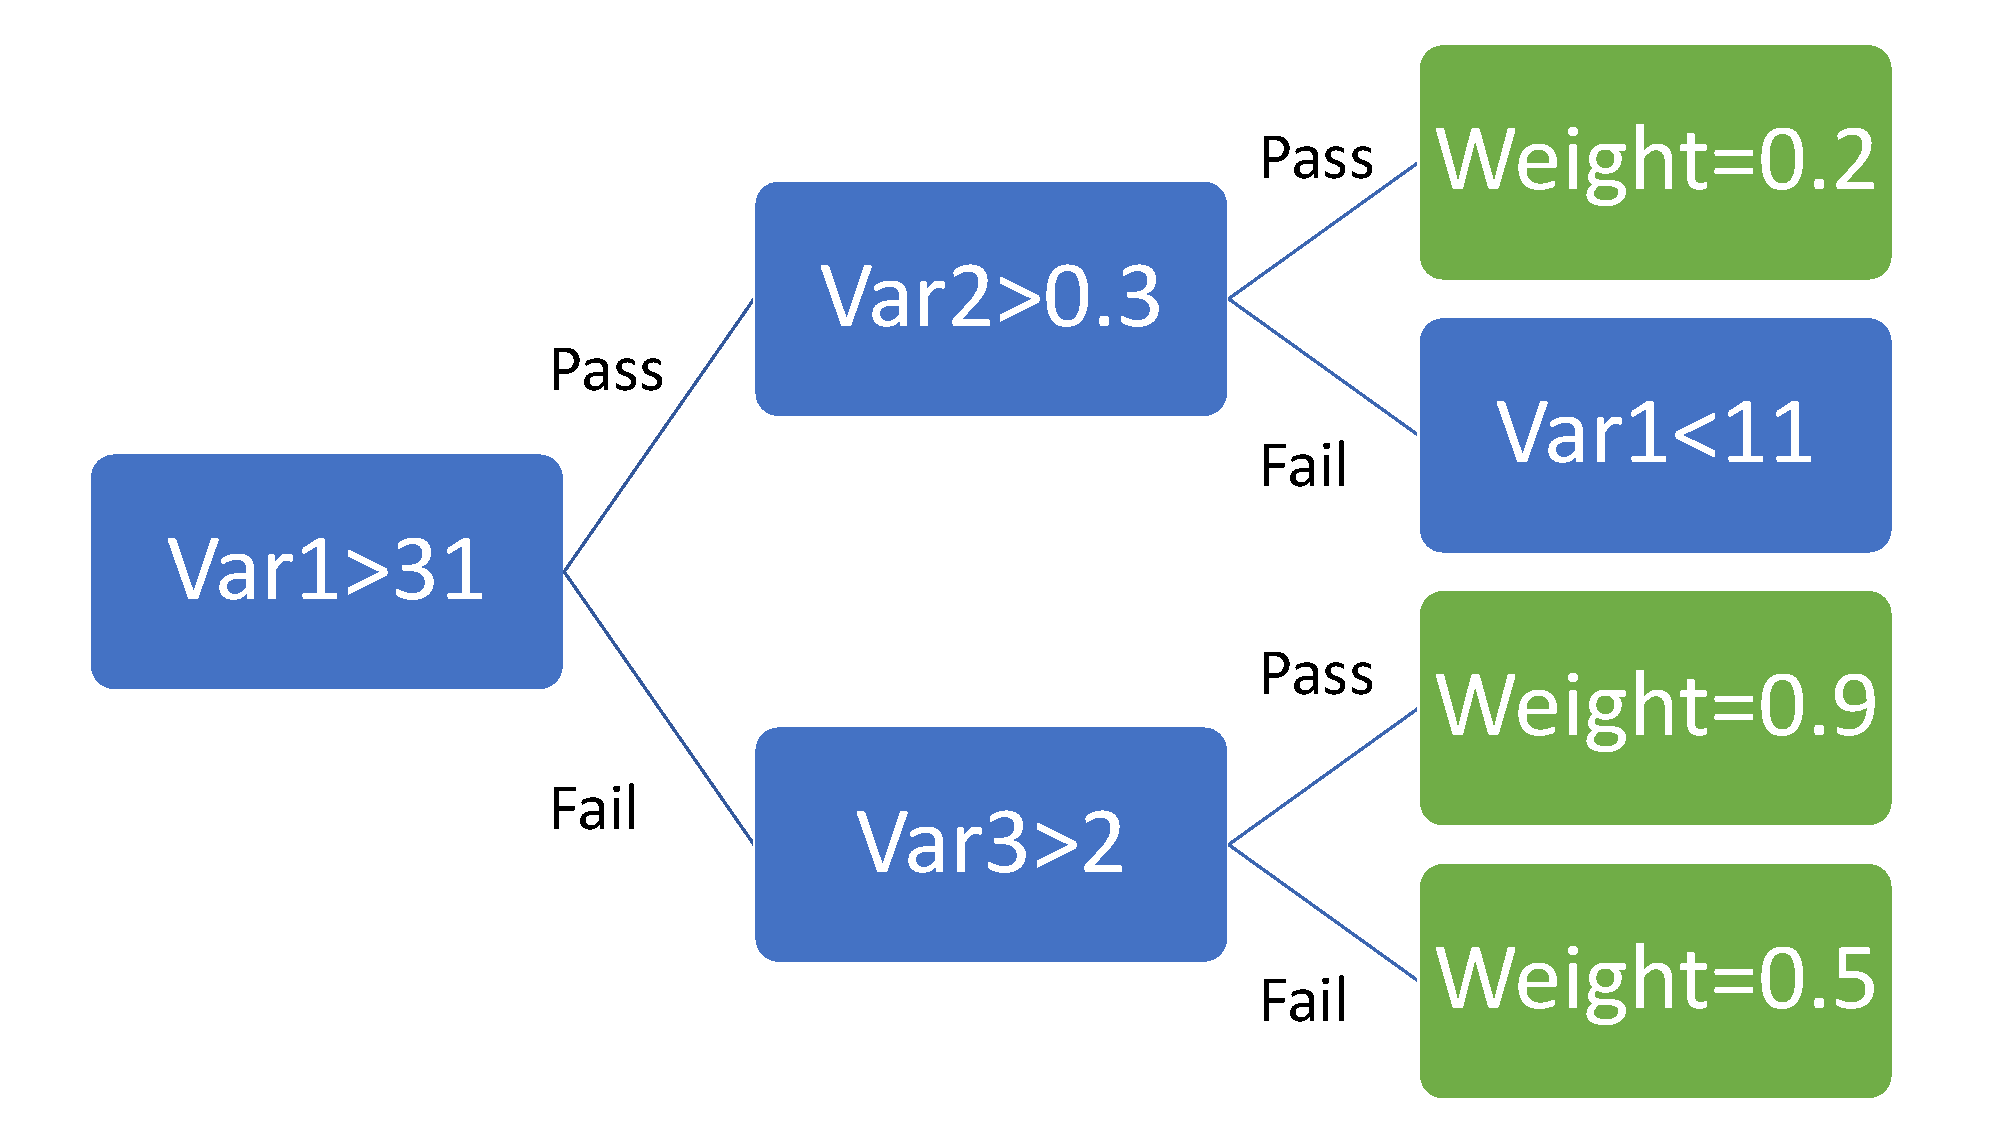
\includegraphics[width=0.78\textwidth,keepaspectratio]{HiggsAnalysis/figures/decisiontree}
  \caption[Example of a decision tree]{Example of a decision tree. Blue represents nodes while green represents leaves}
  \label{fig:decisiontree}
\end{figure}

Following the preselection, the main event selection is then performed using a multivariate approach that takes into account correlations between variables to maximise use of the information available for background discrimination. A \ac{BDT}, implemented in ROOT TMVA \cite{2007physics...3039H} was used for performing this stage of the selection. A detailed description of how a BDT works is given in \cite{Coadou:2013lca}. Fundamentally a decision tree can be represented as a logic flow diagram that assigns a weight to an event based on a series of cuts e.g. see \reffig{fig:decisiontree}. Each level of the flow chart is made up of nodes and leaves. A node represents a cut on a particular variable where the specific value of the cut is chosen to provide the greatest separation between signal and background. A leaf on the other hand represents an end point at which a weight (typically chosen to be the purity of events reaching that point) is assigned to the event. The choice of whether to create a leaf or node after each branching is decided by a stopping criteria. Typically this criteria represents achieving a sufficienctly high purity of signal or background events that the node can be assigned to contain almost entirely signal or background. Typically not all events will have signal like properties for every variable used. As a result it is normally necessary to produce multiple trees (creatively referred to as a forest) using different combinations of variables for each of the nodes. The sum of weights from all the trees used then forms a final discriminating variable for distinguishing between signal and background events. Boosting is then a way of maximising the performance of the decision trees. The simplest form of boosting is to train a set of trees, T$_1$, using a sample of N events. A second set of trees, T$_2$, are then trained using a further N events, half of which were misclassified by T$_1$. A third set of trees, T$_3$,  can then be formed by training on events in which T$_1$ and T$_2$ disagree on the classification. The overall classification is then decided by a democratic vote from T$_1$, T$_2$ and T$_3$. This method yields an improvement in the performance by focusing the training on events that are the hardest to classify correctly. The method can be extended to an arbitrary number of levels T$_N$ where the final \ac{BDT} score is then a weighted sum of the scores from the N trees. By implementing the preselection cuts before training the \ac{BDT}, the overall background rejection is found to be further improved as again, the \ac{BDT} is able to focus only on those events that are hardest to discriminate. Within TMVA, the default parameters for the training are 850 trees per forest with each tree having a maximum depth of three nodes. This provides a balance between the computational time required to train the classifier and the performance it can achieve. However, it is possible an improved performance might be achieved by increasing the number of trees per forest or the depth of each tree. 

The \ac{BDT} in this analysis used 7$\times$10$^4$ signal events and 4$\times$10$^6$ background events, split evenly between training and testing samples. A collection of 19 variables is used for the training:

\begin{itemize}
\item Masses of the reconstructed Higgs and W bosons
\item Energy of the W boson
\item Total missing energy and transverse momentum of the event
\item Number of loose selected isolated leptons
\item PID of the isolated lepton
\item Transverse momentum of lepton
\item Angle of lepton and W boson relative to the beam axis
\item Magnitude of thrust minor observable
\item Number of \ac{PFO}s in the two jets
\item Average angle of the two jets relative to the beam axis
\item kt jet resolution parameter y$_{12}$ (the jet resolution parameter, $d_{ij}$, at which the algorithm transitions from identifying 1 jet in an event to identifying 2)
\item Number of tightly selected PFOs in the event
\item Angular separation of the isolated lepton and reconstructed W boson
\item Minimum angular separation and transverse momentum of the lepton relative to either jet
\item Combined b-tag value for both jets
\end{itemize}

The signal and background distributions for every input variable after application of the preselection cuts can be seen in Appendix A, and the resulting BDT classifier output can be seen in \reffig{bdt}. Of the variables considered, those offering the greatest signal and background were found to be the masses of the Higgs candidate and W boson, the missing energy and the number of isolated leptons in the event.

\begin{figure}
  \centering
  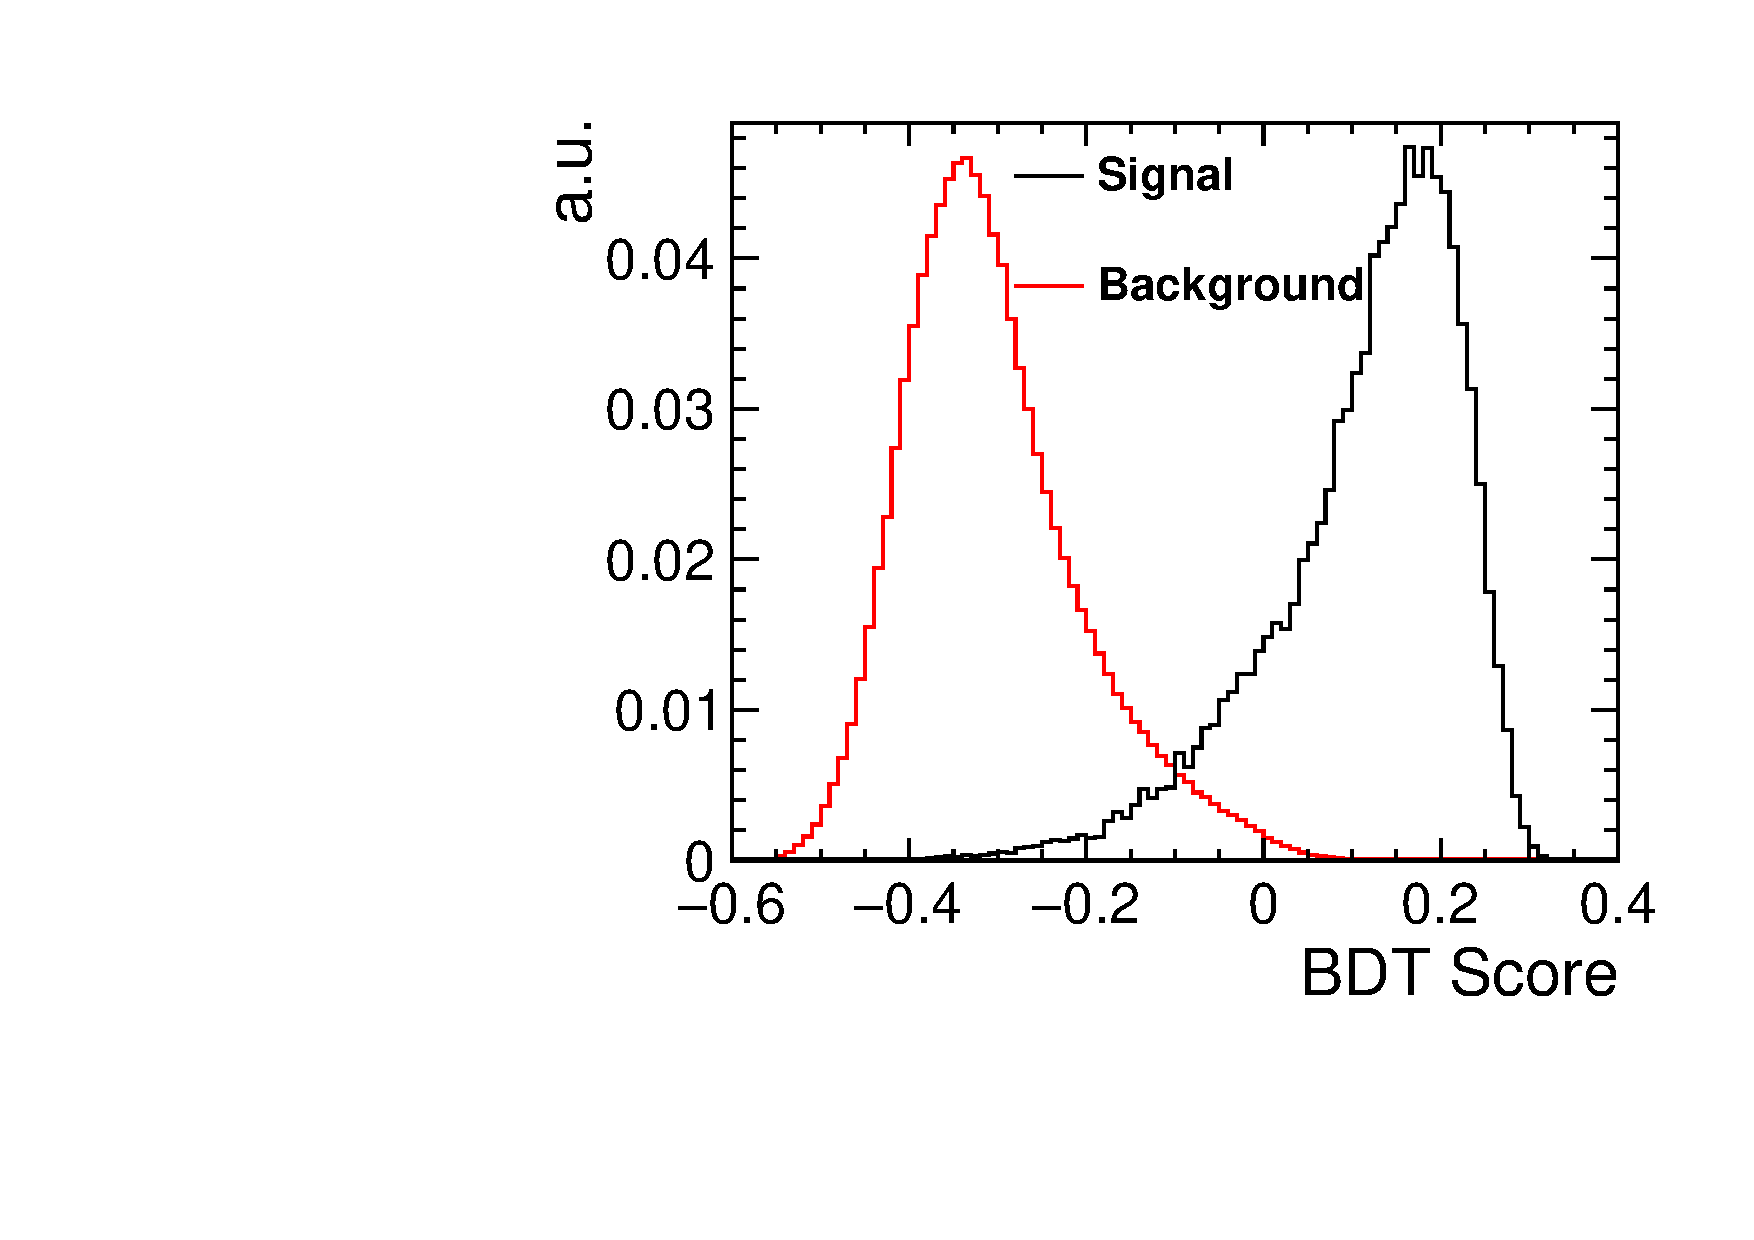
\includegraphics[width=0.78\textwidth,keepaspectratio]{HiggsAnalysis/figures/bdtscore}
  \caption[Classifier BDT response]{BDT response for signal and background events after TMVA classification. Each distribution is normalised to unity.}
  \label{bdt}
\end{figure}

\reffig{bdt} shows that there is a high degree of separation achieved between signal and background events. The efficiencies and number of expected events for signal and background processes for 1.5 ab$^{-1}$ of data following the full event selection are shown in \reftab{tab:finalHiggsResults}. The choice of cut on the BDT score was initially chosen to maximise the signal significance ($S/\sqrt{S+B}$) as this corresponds to the lowest statistical uncertainty on $\sigma\times$BR. Doing this it was found that a maximum significance of 77 was possible by applying a cut on the BDT score of 0.15, corresponding to a statistical uncertainty of 1.30\% on $\sigma\times$BR. However, after later considerations of the relevant systematic uncertainties associated with the measurement (see \refsec{higgsSystematics}), it was found that the overall uncertainty could be reduced by imposing a harsher cut of 0.17 on the BDT score resulting in a slightly larger statistical uncertainty of 1.34\% on $\sigma\times$BR assuming an integrated luminosity of 1.5 ab$^{-1}$. 

This value is similar to that observed for the WW$\rightarrow$qqqq final state, 1.5\%, as expected. By neglecting the case where the isolated lepton it a $\tau$, we have reduced the maximum signal yield to two thirds that of the hadronic channel which inherently limits the precision that can be acheived. However, due to the lack of an easily identifiable isolated charged lepton and the ambiguity associated with assigning the four jets to the two W's, the signal in the qqqq channel is more challenging to distinguish from background events.

Looking in detail at the backgrounds after our selection, we can see that many of the backgrounds have been almost completely removed leaving only ee$\rightarrow$ H($\rightarrow$ other)$\nu\nu$ and ee$\rightarrow$qql$\nu$ as the dominant backgrounds. This is to be expected as these events most closely mimic our signal, which is mainly distinguished by its large missing energy. In the case of H$\rightarrow$other events it was determined that 26\% of the remaining events came from H$\rightarrow\tau^+\tau^-$ processes with a further 25\% from H$\rightarrow$WW* processes with one or more of the Ws decaying to a $\tau$. As such, attempts were made to veto $\tau$ events by rejecting those in which one or more hadronically decaying $\tau$ was explicitly identified using the default ILCSoft Tau Finder \cite{TauFinder} package. However, the misidentification probability for $\tau$s in the signal channel was sufficiently high that the overall statistical uncertainty on $\sigma \times$BR increased and therefore $\tau$ identification is not used in the final selection. It is anticipated that when \ac{CLIC} is commisioned, an updated version of the tau finder package would be developed. One obvious improvement that could be made would be to include particle ID information as determined from Pandora for identifying $\tau$s. With a sufficiently performant $\tau$ finder, up to 50\% of the current backgrounds could potentially be removed. 

The efficiency for selecting WW$^*\rightarrow$qqqq events in the WW$^*\rightarrow$qql$\nu$ channel has been calculated to be 0.2\%. The converse efficiency for selecting WW$^*\rightarrow$qql$\nu$ events in the WW$^*\rightarrow$qqqq channel is 1.0\% which should be sufficiently low that a straightforward combination of the uncertainties determined by both channels can be made. The resulting combined statistical uncertainty on $ee\rightarrow H\nu\nu, H\rightarrow WW^*$ is expected to be $\sim$1.0\%.

\begin{table}
  \centering
  \begin{tabular}{l c c c c}
   \toprule
    Process & Cross Section & Pre-selection & BDT Cut  & Events After BDT     \\
    & (fb) & Eff. & Eff. &      \\
    \midrule
    \midrule
    \bf{ee$\rightarrow$H$\nu\nu$;}            & \bf{17.3}    &  \bf{8.93E-01}  & \bf{3.63E-01} & \bf{9409}    \\
    \bf{H$\rightarrow$WW$^*\rightarrow$qql$\nu$} & & & & \\
    \midrule
    \midrule
    ee$\rightarrow$H$\nu\nu$;  & 27.4    & 4.12E-02 & 2.03E-03 & 84  \\
    H$\rightarrow$WW$^*\rightarrow$qqqq & & & & \\
    ee$\rightarrow$H$\nu\nu$; & 199.4 & 2.64E-01 & 6.93E-03 & 2072 \\
    H$\rightarrow$Other & & & & \\
    \midrule
    \midrule
    ee$\rightarrow$qq               & 4009.5    & 7.21E-02 &  1.72E-05 & 103  \\ 
    ee$\rightarrow$qqqq               & 1328.1    &  2.09E-02 & 3.37E-05 & 67   \\ 
    e$\gamma$$\rightarrow$eqq ($\gamma$ from EPA)                 & 32308    & 7.32E-02  & 1.26E-05 & 612  \\ 
    $\gamma$e$\rightarrow$eqq ($\gamma$ from BS)               &  56043   & 8.02E-02 & 4.54E-06 & 382  \\ 
    ee$\rightarrow$qq$\nu\nu$               & 787.7    & 9.18E-02 & 3.41E-04 & 403   \\ 
    ee$\rightarrow$qqll               & 2725.8    & 1.36E-01  & $<$1.93E-05 & 79    \\ 
    ee$\rightarrow$qql$\nu$              & 4309.7    & 7.90E-02  & 4.20E-04 & 2716    \\ 
    \midrule
    \midrule
    \bf{Total Bkg}                    & \bf{101738.6} & \bf{7.82E-02} & \bf{4.27E-05} & \bf{6518} \\
    \midrule
    \bottomrule
  \end{tabular}
  \label{tab:finalHiggsResults}
  \caption[Samples Used]{Efficiency for all processes following pre-selection and BDT response cuts and the number of events expected to satisfy these requirements, for an integrated luminosity of 1.5 ab$^{-1}$. The MC statisitcal uncertainty on the predicted number of events for the signal and dominant background processes is $\mathcal{O}$(1-5\%). In the case of $e\gamma$ processes the uncertainty is $\mathcal{O}$(50\%) due to their extremely large cross sections.}
  \label{cuts}
\end{table}

\section{Systematics}
\label{higgsSystematics}
On top of the statistical uncertainty there will also be systematic uncertainties on the measurement. These primarily arise because to perform the $\sigma_{H\nu\nu}\times BR_{H\rightarrow WW}$ measurement we must first subtract any residual backgrounds and correct for finite signal efficiency, before finally scaling by the WW$\rightarrow$qql$\nu$ branching ratio. The potential sources of systematic uncertainty that have been identified are as follows:

\textbf{Luminosity}-- At \ac{CLIC} it is estimated that the luminosity can be measured to 0.3\%. Deviations from the nominal value will cause two problems. Firstly the cross section measurement itself will be directly effected as $\sigma=N/L$. Secondly, the number of background events recorded will differ from that which is predicted. As a result the background subtraction will either no longer remove all the background or will remove all the background but also remove some signal events too. The effect of the luminosity uncertainty was quantified by varying the total number of events after event selection by $\pm$ 0.3\% before background subtraction and efficiency corrections then measuring the variation seen in the measured cross section. This resulted in an uncertainty of 0.51\% on $\sigma_{H\nu\nu}\times BR_{H\rightarrow WW}$.

\textbf{Background Normalization}-- In order to remove the backgrounds remaining after the event selection, a precise knowledge of the overall background normalization is required. For all background processes there will be an uncertainty associated with their cross section. To evaluate the effect of these uncertainties, the number of events selected from each background process were varied independently and the resulting change in $\sigma_{H\nu\nu}\times BR_{H\rightarrow WW}$ was determined. The uncertainties from changing each of the backgrounds individually were then added in quadrature to obtain the total uncertainty on the background normalization. In the case of Higgs related backgrounds a fluctuation of 5\% was used for the normalization. This value was motivated by the studies presented in  \cite{Abramowicz:2016zbo} where a statistical uncertainty of $\mathcal{O}$(5\%) is expected on the dominant Higgs decays modes for Higgs produced through WW-fusion at 1.4 TeV. For the remaining backgrounds, fluctuations of the order 1\% were used. Overall this is found to give a combined uncertainty of 1.14\% on $\sigma_{H\nu\nu}\times BR_{H\rightarrow WW}$ making it the dominant systematic effect. The minimization of this uncertainty is the basis for increasing the requirements imposed on the BDT response. Selecting the BDT score that minimised the statistical uncertainty was found to give a systematic uncertainty from the background normalization of $\mathcal{O}$(2\%) due to a larger total number of backgrounds passing the event selection. Hence we see that for a small degredation in the statistical uncertainty we gain a large improvement in the systematic uncertainty.

\textbf{W Branching Ratios}-- In order to measure $\sigma_{H\nu\nu}\times BR_{H\rightarrow WW}$ it is necessary to correct for the $WW\rightarrow qql\nu$ branching ratio. This quantity is already well measured\cite{Patrignani:2016xqp} with an uncertainty of 0.09\% (0.27\%) for the leptonc (hadronic) decay modes. This gives an uncertainty on the branching ratio $WW\rightarrow qql\nu$ and $\sigma_{H\nu\nu}\times BR_{H\rightarrow WW}$ of 0.57\%.

As well as these uncertainties there are other effects that have not yet been quantified. In particular, it would be beneficial to examine the effect of using a different event generator/hadronization scheme to evaluate the effect of modelling on the variables used in the event selection. However, there are currently no alternative simulation packages available within the linear collider framework and so there is currently no quantification of these effects. Overall it is believed that the effect of different hadronization models should be small when compared to the other systematic effects as few of the input variables for training the BDT are expected to be sensitive to modelling effects.

Detector effects such as the lepton and jet reconstruction efficiencies are not considered here as they cannot be reliably evaluated without an existing detector, however they should be accounted for once the detector has been built and tested.

Combining the various systematic effects leads to a total systematic uncertainty of 1.37\%. This is of the same order as the statistical component (1.34\%.) Ultimately it is expected that these values probably represent an overestimate of the performance that \ac{CLIC} will achieve as advances in analytical techniques will likely occur over the time scale ($\sim$ 20 years) before this measurement would actually be performed allowing for improved event reconstruction and background rejection leading to reduced statistical and systematic uncertainties.  

\section{Impact on CLIC Higgs Measurements}
As discussed at the start of this chapter, the main motivation behind performing this measurement is to allow the Higgs width to be determined so that model independent measurements of the Higgs couplings can be performed. As a result we should look at this measurement in terms of the other measurements required for measuring the Higgs width.

\begin{table}
  \centering
  \begin{tabular}{c c }
   \toprule
    Process & Statistical Precision at 1.4 TeV (\%)    \\
    \midrule
    $X_1=\sigma_{ZH} \propto g_{HZZ}^2$ & 1.7 \\
    \midrule
    $X_2=\sigma_{H\nu\bar{\nu}} \times BR(H\rightarrow WW^*) \propto \frac{g_{HWW}^4}{\Gamma_H}$ & 1.0\\
    \midrule
    $X_3=\sigma_{H\nu\bar{\nu}} \times BR(H\rightarrow b\bar{b}) \propto \frac{g_{HWW}^{2}g_{Hbb}^2}{\Gamma_H}$ & 0.4\\
    \midrule
    $X_4=\sigma_{ZH} \times BR(H\rightarrow b\bar{b}) \propto \frac{g_{HZZ}^{2}g_{Hbb}^2}{\Gamma_H}$ & 0.9 \\
    \bottomrule
  \end{tabular}
  \caption[Expected precision on input quantites for the Higgs width measurement]{Expected precision on input quantites for the Higgs width measurement\cite{Abramowicz:2016zbo}. The value for $X_2$ represents the precision obtainable when combining the results presented in this chapter with those of the ee$\rightarrow$ H(WW$^*\rightarrow$qqqq)$\nu\nu$ channel analysis.}
  \label{fig:higgscomparison}
\end{table}

One can see from \reftab{fig:higgscomparison} that the measurements presented above are sufficiecntly performant that the width measurement is not limited by the $\sigma_{H\nu\nu}\times BR_{H\rightarrow WW}$ measurement, instead it is limited by the precision on the higgstrahlung cross section as measured during the low energy run. Overall, combining the measurements an statistical uncertainty of 3.7\% is expected on the Higgs width at 1.4 TeV for 1.5 ab$^{-1}$ of data.

\section{Conclusion}

In summary, we have performed a full analysis of the ee$\rightarrow$ H(WW$^*$)$\nu\nu$, WW$^*\rightarrow$qql$\nu$ decay channel using a large set of simulated backgrounds with the aim of measuring the H$\rightarrow$WW$^*$ branching ratio as input for a model independent measurement of the total Higgs width. A 19 variable BDT was used to select signal events where the final state charged lepton is either an electron or a muon, and to remove background events. These backgrounds were found to be dominated by ee$\rightarrow$ H($\rightarrow$ Other)$\nu\nu$  and ee$\rightarrow$qql$\nu$ in the final selection. Several systematic effects have been considered, with the dominant uncertainty coming from the background normalization. The resulting uncertainty for 1.5~ab$^{-1}$ of data at 1.4~TeV was found to be: \\[10pt]\centerline{\large{$\Delta\sigma_{H\nu\nu}$ x BR(H$\rightarrow$WW$^*$) = 1.34\%$_{Stat} \oplus$ 1.37\%$_{Syst}$}} \\[10pt] The efficiency for incorrectly selecting ee$\rightarrow$H(WW$^*$)$\nu\nu$, with WW$^*\rightarrow$qqqq, in the WW$^*\rightarrow$qql$\nu$ channel, was found to be 0.2\%. The correlated overlap in selections developed for the WW$^*\rightarrow$qqqq and WW$^*\rightarrow$qqlv final states would be taken into account when combining the individual results, however the combined statistical precision is expected to be 1.0\%. Combining this with the other proposed measurements at 1.4~TeV and the low energy stage at CLIC yields an overall statistical precision of 3.7\% on the total Higgs width\cite{Abramowicz:2016zbo}.



